\documentclass[9pt,tutorial]{livecoms}
%\documentclass[10pt,twocolumn]{article}


\usepackage[version=4]{mhchem}
\usepackage{siunitx}
\DeclareSIUnit\Molar{M}
\usepackage[italic]{mathastext}
\graphicspath{{Figures/}}
\usepackage{natbib}
\usepackage{enumitem}
\usepackage{hyperref}
\usepackage{listings}
\hypersetup{
    colorlinks=true,
    linkcolor=blue,
    filecolor=magenta,      
    urlcolor=cyan,
    pdftitle={Overleaf Example},
    pdfpagemode=FullScreen,
    }

% \newcommand{\versionnumber}{0.1}  % you should update the minor version number in preprints and major version number of submissions.
% \newcommand{\githubrepository}{\url{https://github.com/myaccount/homegithubrepository}}  %this should be the main github repository for this article

\newcommand{\jh}[1]{\textcolor{blue}{JH: #1}}
\newcommand{\grace}[1]{\textcolor{red}{GB: #1}}
\newcommand{\Mina}[1]{\textcolor{magenta}{Mina: #1}}

\title{Computing absolute binding affinities by Streamlined Alchemical Free Energy Perturbation}
% :\\ a Tutorial [Article v\versionnumber]

\author[1,2,3]{Mina Ebrahimi}
\author[4]{Grace Brannigan}
\author[2,3]{Jérôme Hénin}
\affil[1]{Department of Physical Chemistry, School of Chemistry, College of Science, University of Tehran, Tehran, Iran.}
\affil[2]{CNRS, Université de Paris, UPR 9080, Laboratoire de Biochimie Théorique, 13 rue Pierre et Marie Curie, 75005, Paris, France}
\affil[3]{Institut de Biologie Physico-Chimique -- Fondation Edmond de Rothschild, PSL Research University, Paris, France}
\affil[4]{Rutgers University, Camden, New Jersey, 08102}

\corr{henin@ibpc.fr}{JH}

% \orcid{Author 1 name}{AAAA-BBBB-CCCC-DDDD}
% \orcid{Author 2 name}{EEEE-FFFF-GGGG-HHHH}



% \blurb{This LiveCoMS document is maintained online on GitHub at \githubrepository; to provide feedback, suggestions, or help improve it, please visit the GitHub repository and participate via the issue tracker.}

%%%%%%%%%%%%%%%%%%%%%%%%%%%%%%%%%%%%%%%%%%%%%%%%%%%%%%%%%%%%
%%% PUBLICATION INFORMATION
%%% Fill out these parameters when available
%%% These are used when the "pubversion" option is invoked
%%%%%%%%%%%%%%%%%%%%%%%%%%%%%%%%%%%%%%%%%%%%%%%%%%%%%%%%%%%%
% \pubDOI{10.XXXX/YYYYYYY}
% \pubvolume{<volume>}
% \pubissue{<issue>}
% \pubyear{<year>}
% \articlenum{<number>}
% \datereceived{Day Month Year}
% \dateaccepted{Day Month Year}

\begin{document}

\begin{frontmatter}
\maketitle

\begin{abstract}
This tutorial describes the double decoupling approach using alchemical free energy perturbation (AFEP) to reproduce the experimental ligand affinity. A wide range of in silico ligand affinity predictions are performed using the AFEP method, this tutorial is built around the Streamlined AFEP (SAFEP) approach, which uses distance-from-bound-configuration (DBC) restraints in the Colvars Module. DBC restraints limit the ligand's conformational changes as well as roto-translational movement relative to the protein to their unbiased fluctuations in the bound state. In the following, the binding free energy of phenol to a mutant lysozyme (L99A/M102H) is estimated using this innovative sampling framework.
\end{abstract}

\end{frontmatter}

\section{Introduction}

\section{Scope}
This tutorial covers the calculation of absolute binding affinity through computational alchemy, traditionally known as Free Energy Perturbation (FEP). Here, we use a simple and site-centered approach, which relies on a single recently-introduced collective variable to define the binding site and achieve robust convergence. This flavor of FEP is known as Streamlined Alchemical Free Energy Perturbation (SAFEP) \cite{Salari2018}.

\section{Prerequisites}

\subsection{Background knowledge}\label{sec:7.1}

It is assumed that users are familiar with standard molecular dynamics simulation using NAMD package. Otherwise, please explore these two tutorials: “NAMD Tutorial” \cite{phillips2003} and “In silico alchemy: A tutorial for alchemical free-energy perturbation calculations with NAMD” \cite{Henin2017}. Also, basic knowledge of using VMD is necessary for visualization, input preparation, and post-processing. While running the steps in the "Cheat Sheet" requires only superficial understanding, adapting these steps to your own system will require more familiarity with TCL. 
%basic knowledge of the Python programming languages is necessary to prepare initial structure, reference files, and running the scripts. 
Furthermore, output analysis concerning with thermodynamic integration method is proceeded by Grace (xmgrace), but many other tools (Python, Matlab, R, Mathematica) can be used alternatively. 
%In summary, 
% users will need: 
% \begin{itemize}[left=0pt .. \parindent]
% \item Knowledge of classical molecular dynamics simulations, and in particular, NAMD.  
% \item Basic knowledge of TCL and python scripting. 
% \end{itemize}
%Tutorials should clearly define what concepts or abilities researchers will need to complete the tutorial (e.g., some proficiency in Python; experience with Jupyter notebooks; knowledge of classical MD; etc).
\subsection{Software requirements}\label{sec:7.2}

NAMD 2.14 or later \cite{Phillips2020} will be used to perform simulations using both CPU or GPU. Note that alchemical transformations are only implemented in the CPU versions of NAMD 2, but NAMD 3.0 introduces alchemy on the GPU \cite{Chen2020}.
In order to monitor, analyze, and visualize the simulations and AFEP outputs, VMD 1.9.4 or later \cite{Humphrey1996} is needed. In the "cheat sheet", the output data post-processing is conducted by a Jupyter notebook (ipynb file) requiring Python 3.0 and the alchemlyb library. 
In summary, the minimal required software is:
\begin{itemize}[left=0pt .. \parindent]
\item NAMD 2.14 or later\cite{Phillips2020}
\item VMD 1.9.4 or later \cite{Humphrey1996}
\item Python 3.0
\item Alchemlyb library \cite{shirts2008statistically, chodera2016simple}
%\item A data analysis or graphing software like xmgrace 
\end{itemize}

%Tutorials should clearly define what system and/or software requirements the researcher will need to complete the tutorial (e.g., VMD version 1.9 or newer, AMBER, etc.). Tutorials requiring specific software packages must provide instructions and files for the referenced version of the software.
%\subsection{Theoretical background}
% The alchemical free energy perturbation (AFEP) method can predict ligand-protein binding affinities efficiently thanks to fictitious intermediate states. A thermodynamic cycle is established through a series of nonphysical transformations between initial and final states. The free energy change {$\Delta G$} around the cycle is zero because the free energy is a state function. \cite{Kollman1993, Chodera2011, Deng2018, Bhati2018, Kuhn2020}.
% Nevertheless, the selection of intermediate states conditions the accuracy and efficiency of the free energy assessment. AFEP with double decoupling is a formally exact approach, but numerical convergence can be difficult to achieve\cite{Pohorille2010}.
% Although an abundance of comprehensive essays are available about the theory of affinity calculations, we briefly review the methodology background \cite{Bhandarkar2009, VanGunsteren2002, Chipot2006}.

% We describe an alchemical transformation from state $A$ to state $B$ through a different Hamiltonian for each state, $H_A$ and $H_B$, and more precisely, potential energy functions $U_A$ and $U_B$ (the kinetic energy does not change, and cancels out of the free energy calculations).

% The difference of free energy between two arbitrary states (say, a reference $r$ and a target $t$) can be calculated \textit{exactly} by the exponential formula:\cite{Zwanzig1954}
% \begin{align}\label{eq:exp_formula}
% \Delta F_{r\rightarrow t} &= -\frac{1}{\beta}\ln{ \left\langle \frac{e^{-\beta U_t(q, p)}} {e^{-\beta U_r(q, p)}}
% \right\rangle}_r \\
% &= -\frac{1}{\beta}\ln{ \left\langle e^{-\beta\Delta U_{r\rightarrow t}(q, p)} \right\rangle}_r
% \end{align}
% where $\beta$ is the inverse temperature $1/(k_B T)$, and the bracket indicates an average over $(q, p)$ in the canonical ensemble for the potential energy $U_r$, that is, an \textit{average in the reference state}.
% For any non-trivial perturbation, the exponential average in Eq.~(\ref{eq:exp_formula}) converges excruciatingly slowly, making this expression less than useful.
% In practice, to improve numerical convergence, the transformation from the reference to the target state is split into smaller steps, connecting a series of nonphysical intermediate states \cite{Beveridge1989}.
% Thus we can apply Eq.~(\ref{eq:exp_formula}) to many intermediate states between $A$ and $B$.

% The perturbation can be described continuously by a potential energy that depends on a “coupling parameter” $\lambda$ between 0 and 1.
% In the simplest case, it is a linear combination of the initial and final state potential energies:
% \begin{equation}\label{eq:U_lambda}
% U_\lambda(q, p)=(1-\lambda)U_A(q, p)+\lambda U_B(q, p)
% \end{equation}

% Calculating the difference of a free energy between the states through a series of intermediate transformations makes the exponential formula converge faster.
% There are also estimators termed \textit{Overlap Sampling} that improve convergence by introducing fictitious intermediate sates with better overlap with the states of interest and using them as target state in the exponential formula.
% These include simple overlap sampling (SOS) and Bennett's acceptance ratio (BAR). The SOS strategy simulates forward and a reverse sampling to an intermediate halfway between $\lambda_i$ and $\lambda_{i+1}$:\cite{Lu2004}
% \begin{equation}\label{eq:SOS}
% \Delta F_{i,i+1}=-\frac{1}{\beta}\ln{\frac
% {\left\langle e^{-\beta\Delta U_{i,i+1}/2} \right\rangle_{i}}
% {\left\langle e^{\beta\Delta U_{i,i+1}/2} \right\rangle_{i+1}}
% }
% \end{equation}
% BAR determines the optimal intermediate state by an iterative procedure, minimizing the statistical error\cite{Bennett1976,Lu2004,Lu2004a}.


% Thermodynamic integration is an alternative general-purpose method for the calculation of free energies along a continuous parameter, which may be a geometric coordinate or an alchemical coupling parameter. \cite{Mitchell1991,VanGunsteren2002,Jorge2010} 
% Thermodynamic integration can be written as:
% \begin{equation}\label{eq:TI}
% \Delta F=\int_0^1\left\langle\frac{\partial U_\lambda(q,p)}{\partial\lambda}\right\rangle_\lambda d\lambda
% \end{equation}

% In all alchemical transformations where particles are annihilated or decoupled from the environment, a singularity problem referred to as “end-point catastrophe” can occurred at the end points where repulsive nonbonded interactions disappear.
% With linear scaling of the repulsive potential, the free energy derivative with respect to $\lambda$ is infinite at the end-points, making the free energy estimation unreliable.
% To avoid this singularity, the interaction potential energy is transformed as a nonlinear function of $\lambda$, to behave as a so-called “soft-core potential” \cite{Beutler1994,Zacharias1994}.

% In the double decoupling method (DDM), the ligand is decoupled separately from the binding site and from bulk solution, by turning off the ligand's van der Waals and electrostatic interactions \cite{Straatsma1992, Boresch2003, Nishikawa2018}.
% Restraining potentials are usually applied to the ligand in the binding cavity to prevent it from diffusing away from the site and sampling a large volume of irrelevant configurations when it becomes mostly decoupled\cite{Deng2009}.
% It is necessary to account for the effect of the restraining potential when computing the standard free energy of binding.
% This contribution can be estimated numerically by a restraint free-energy perturbation (RFEP) simulation.\cite{Mobley2006, Deng2009, Salari2018, Sakae2020}.

\section{Content and Links}

\subsection{Cheat Sheet}
Follow the steps below for a basic calculation of the binding affinity of phenol to lysozyme. More detail on the rationale for each step, as well as alternative options, can be found in the hyperlinked sections. All supporting files are provided in the \href{https://github.com/jhenin/SAFEP_tutorial}{SAFEP$\_$tutorial repository}. In commands of this material, replace the \texttt{user$\_$dir} with the directory that you unzip the \texttt{Supp-Files} contents.

The steps below assume that you already have a solvated system prepared for basic MD simulation. We provide these files for the tutorial, and details of how they were prepared are in \hyperref[sec:6.1]{System Preparation}.

\begin{enumerate}[left=0pt .. \parindent]
     \item {\hyperref[sec:8.2]{\bf Defining the occupied state}}~
     \begin{enumerate}
     \item Load the "solv-prot.psf" and "solv-prot.pdb" into vmd.
     %\item Choose which protein atoms define the protein site. Here we will use the alpha carbons that are within 14 {\AA} of the bound ligand. Open the TkConsole and enter the following tcl code to get the atoms serial numbers: 
      % \grace{use of the colvars dashboard makes this step unnecessary doesn't it?}\Mina{Yes, this step would be done in the step (c)}
%\begin{verbatim}
%[atomselect top "alpha and within 14 of 
%resname PHEN"] get serial
%\end{verbatim} 
%Open the dbc colvar template in a text editor and copy the atom numbers from the previous step into the fittingGroup section of the dbc colvar template: 
     \item Open the Colvars Dashboard through VMD main menu$\rightarrow$Extensions$\rightarrow$Analysis$\rightarrow$Colvars Dashboard, then click "Edit" to edit a new collective variable.
Load the "DBC ligand RMSD" template from the left panel drop-down menu: "Templates/colvar templates".

     \item Define the atom selection for the ligand atoms:
Delete the "\texttt{atomNumbers 1 2 3 4}" line following the comment "\texttt{$\#$Define ligand atoms}".
In its place, insert the atom numbers of all heavy atoms of the ligand by entering "\texttt{resname PHEN and noh}" into the text box "Editing helpers/atoms from selection text" in the left panel, then press Enter to insert the new selection into the configuration text.

     \item Similarly, define the binding site atoms:
Replace the "\texttt{atomNumbers}" line within the "\texttt{fittingGroup}" block with the atom numbers corresponding to the selection text "\texttt{alpha and within 14 of resname PHEN}".

% \item In the "DBC ligand RMSD" template, insert the atom selection in the "fittingGroup" block using the Colvars config editor to get the input configuration.
% The DBC-unbiased.colvars, the Colvars input file, is provided in details in Section \ref{Section 6.2.2}. 
%\grace{JH I think we still need instructions on what they should actually do.}
%\jh{I think it's clearer now}
%\item Copy the resulting atom numbers into the dbc colvar template:
%\begin{verbatim}
%  atoms {
%  # Define ligand atoms used for RMSD calculation
%    atomNumbers <ligand atoms>
%\end{verbatim}

\item Create the file containing the reference coordinates for the ligand and binding site  (rest-ref.pdb, which is distinct from solv-prot.pdb), by entering the following lines in VMD TkConsole:
\begin{verbatim}
[atomselect top all] set occupancy 0
[atomselect top "(alpha within 14 of resname PHEN) 
or (resname PHEN and noh)"] set occupancy 1
[atomselect top all] writepdb rest-ref.pdb
\end{verbatim}
\item Edit the "DBC ligand RMSD" template within the Colvars dashboard editor to point to the reference pdb file that you wrote in the previous step, by changing the default line
\begin{verbatim}
refpositionsfile reference.pdb
\end{verbatim} 
to 
\begin{verbatim}
refpositionsfile rest-ref.pdb
\end{verbatim} 
Note that you need to do this for both instances of the keyword (one in the atom group, and one in the RMSD block) and press "Apply[Ctrl-s]".
In the Colvar dashboard main menu, click on "Save colvars" at the top, change to the directory and save the "DBC ligand RMSD" as the "DBC-unbiased.colvars".
Optional: You can set the output files frequencies by using "colvarsTrajFrequency" and "colvarsRestartFrequency" keywords in the "DBC ligand RMSD" input file.
\item Open the "DBC-unbiased.colvars" in a text editor, add a separate block for the histogram feature, with the following content:
\begin{verbatim}
histogram {
  colvars DBC
  outputFile DBC.dat
  histogramGrid {
    widths          0.1 
    lowerboundaries 0.0
    upperboundaries 10.0
  }
}
\end{verbatim}
% Use \href{https://colvars.github.io/colvars-refman-namd/colvars-refman-namd.html}{Colvars Reference manual} adding histogram block into the "DBC ligand RMSD" template. Conveniently, you can follow the instruction in section \ref{section 6.3.1}. Keep in mind to set "smp" off in the "DBC ligand RMSD" input file by inserting the command line as follows: 
% \begin {verbatim}
%  smp off
% \end{verbatim}
% First, you must change the directory of the VMD TK console to where rest-ref.pdb file is saved.
% Then, click "Apply [Ctrl-S]" to apply changes.

%\grace{Click "Apply [Ctrl-S]" to write out the DBC file? Do they need to save it to a specific place?}

%You can delete any comment you don't need (anything after a "$\#$" character). 
\item Run unbiased, traditional MD of the occupied state using the configuration files provided. Look out! The unbiased simulation is a long equilibration (at least 50 ns in this material) for exploratory analysis, predicting the tolerance of the DBC ligand for all bound modes. The short simulation might lead to a false evaluation.
\begin{verbatim}
user_dir/Supp-Files/DBC-Unbiased/namd2
  equ.namd
\end{verbatim}
Note: the equilibration included in the unbiased simulation is specifically necessary for this material and can be skipped for other examples. The rationale is provided in section \ref{section 6.4}.
\begin{verbatim}
user_dir/Supp-Files/DBC-Unbiased/namd2
  run.namd
\end{verbatim}
\item The output of the histogram will be in the DBC.dat file. View the histogram using your own preferred tool, or run 
\begin{verbatim}
user_dir/Supp-Files/DBC-Unbiased/outputs/python
  1-Plot-histogram.py
\end{verbatim}
Bear in mind that Colvar-grid.py will be called as a class by "1-Plot-histogram.py" script.
\item From the histogram, determine the DBC tolerance such that it is larger than at least 95\% of the RMSD values (95 percentile or greater).  
\item From the \href{https://colvars.github.io/colvars-refman-namd/colvars-refman-namd.html}{Colvars Reference manual}, add "Harmonic wall restraints" into the "DBC ligand RMSD" input file and modify the \texttt{upperWalls} parameter corresponds to the DBC tolerance. In the \texttt{harmonicWalls} block, set the \texttt{colvars} keyword the DBC, the name of "DBC ligand RMSD" colvar, and choose an appropriate value for the \texttt{forceConstant} keyword. Please, find the example in section \ref{section 7.1}. %\jh{This is an older Colvars syntax, it should be upperWall now - check the file} \Mina{Yes, exactly it is upperWalls.}
\end{enumerate}
If it is necessary to change atom group definitions after running the equilibrium MD, you can also analyze through post-processing in Section \ref{section 6.3}. 
    
\item {\bf \hyperref[section 7]{Protein Decoupling}}
\begin{enumerate}
\item The atoms which will be decoupled are indicated via the solv-prot-charmm.fep file. These are most conveniently written using VMD. Reload the same solv-prot.psf and solv-prot.pdb (or VMD session) from step 1, and then open the Tkconsole:  
\begin{verbatim}
[atomselect top all] set beta 0
[atomselect top "resname PHEN"] set beta -1
[atomselect top all] writepdb solv-prot-charmm.fep
\end{verbatim}
\item Run the protein decoupling step. The NAMD configuration file will use the colvar inputs that you created in Step 1. 
\begin{verbatim}
user_dir/Supp-Files/AFEP-Bound-Decoupling/namd2
  equ.namd
\end{verbatim}
After equilibration, then perform the production run:
\begin{verbatim}
user_dir/Supp-Files/AFEP-Bound-Decoupling/namd2
  run.namd
\end{verbatim}
\item Open the included ipython notebook\\ BAR\_NAMD\_alchemlyb.ipynb, and run each cell in the workbook using the following stepwise instruction. %First, download the source code of alchemlyb, the updated version for IDWS in NAMD, from \url{https://github.com/ttjoseph/alchemlyb/tree/namdupdates}. Next, extract the source code and copy " .fepout" file and BAR\_NAMD\_alchemlyb.ipynb in the \texttt{/alchemlyb-namdupdates/src} directory.
In the directory containing .fepout" and BAR\_NAMD\_alchemlyb.ipynb files, open the terminal (in Linux and MacOS) or Anaconda Prompt (in Windows), executing the command \texttt{jupyter notebook}. From the directory tree in the jupyter notebook showing up in the web browser, open the BAR\_NAMD\_alchemlyb.ipynb and run all cells from the menu bar through Cell${\rightarrow}$Run All. Note: Python 3.0 and alchemlyb library are necessary for executing BAR\_NAMD\_alchemlyb.ipynb script. 


\item Examine the plot titled ``Distribution of fwd-bwd discrepancies". In a perfect calculation, this distribution would be symmetric and centered around 0. If your distribution is highly skewed or has a mean that is more than one standard deviation away from 0, please see "Diagnosing and addressing convergence problems". Otherwise, please move on to the next step. 
\item Extract the value of  ${\Delta G^*_{site}}$ from the first output list beneath the fifth cell in the ipython notebook, the ${\Delta G}$ concerned with the last sampling at {$\lambda$}=1 exhibits the ${\Delta G^*_{site}}$ in units of kcal/mol.
\end{enumerate}
\item {\bf \hyperref[sec:10]{DBC Restraint Free Energy Correction}}

Run a thermodynamic integration calculation on the ligand in vacuum, releasing the DBC restraint within a spherical restraint of volume $V_0$. 
\begin{enumerate}
\item Choose the radius $R$ of the spherical restraint. It should be much larger (at least twice as large) as the DBC tolerance you identified in Step 1j. Calculate the volume $V_0 = 4/3\pi R^3$.
\item Load the "DBC ligand RMSD" input file into the Colvar dashboard. In the Colvar config editor, insert the "basic colvar" from the drop-down menu: Templates/colvar templates. First, set the "distance" as "name" in the colvar block. Define the atom selection of ligand atoms for the "group1" in the distance block, same as step 1c. Then, in the "group2", replace "\texttt{atomNumbers 2}" with "\texttt{dummyAtom (-2.168, 5.235, 9.367)}", the ligand center position. In the "\texttt{harmonicWalls}" block, change the "DBC" name following the \texttt{colvars} keyword into the "distance", and set the "upperWalls" parameter of the spherical restraint to the radius $R$ to retain the spherical restraint. The completed input file, DBC-Restraint-RFEP.colvars, is provided in /Supp-Files/RFEP. Furthermore, you can find more detail in section \ref{section 6.3.3}.
\item Release the DBC restraint gradually using TI, while retaining the spherical restraint. Practically, the DBC restraint is removed slowly by using a changing flat-bottom harmonic restraint in the DBC-Restraint-RFEP.colvars file. To add the changing harmonic restraint in the "DBC ligand RMSD" input file, please see section \ref{section 8.2}.
\begin{verbatim}
user_dir\Supp-Files\RFEP\namd2  run.namd 
\end{verbatim}
\item Parse the TI output and get the $\Delta G_{DBC}$:
\begin{verbatim}
grep "Lambda="  rfep.log | awk ’{print 
$5, $7*0.025}’ > RFEP.dat
awk -F' ' '{sum+=$2;}END{print -sum;}' RFEP.dat
\end{verbatim}
%\item Plot RFEP.dat and integrate over {$\lambda$} to get $\Delta G_{DBC}$. 

\end{enumerate}
\item  {\bf \hyperref[sec:11]{Decoupling from solvent}}
\begin{enumerate}
\item Equilibrate the ligand in solvent by running
\begin{verbatim}
user_dir\Supp-Files\AFEP-Hydration\namd2
  equ.namd
\end{verbatim}
\item Decouple ligand from solvent
\begin{verbatim}
user_dir\Supp-Files\AFEP-Hydration\namd2
  run.namd
\end{verbatim}
\item Parse the " .fepout" file using the ipython notebook BAR\_NAMD\_alchemlyb.ipynb, as in Step 2c. 
\item Run at least four more replicas to get individual values of $\Delta G^*_{bulk}$, and average them together. 
\end{enumerate}
\item {\bf \hyperref[sec:12]{Calculate corrections and combine  quantities}}
\begin{enumerate}
\item Calculate the ideal gas contribution for your desired concentration [L]:
$$\Delta G_V[L]=-k_B T\ln V_o[L]$$
where $\Delta G_V^\circ \equiv \Delta G_V[1M] = -k_B T\ln V_o/1660$ \AA$^3$.  
\item Use Eq. \ref{eq:delta_G_bind}  to determine $\Delta G_{bind}^\circ$, where $\Delta G^*_{site}$ was calculated in Step 2, $\Delta G_{DBC}$ was calculated in Step 3, $\Delta G^*_{bulk}$ was calculated in Step 4.
%$$\Delta G_{bind}^\circ  = \Delta G^*_{site} + \Delta G_{DBC}-\Delta G^*_{bulk}  + \Delta G_V^\circ$$. 
\end{enumerate}
\end{enumerate}
\section{Overview}
\grace{I renamed this section from ``Practical considerations: ligand restraints"} 
\subsection{SAFEP}
In the conventional DDM, conformational, rotational, and translational degrees of freedom of the ligand relative to the receptor are individually restrained using biasing potentials.
All these restraints affect binding, and their contribution must be calculated to predict the absolute binding free energy \cite{Hermans1997, Gilson1997, Boresch2003, Hamelberg2004, Woo2005, Deng2006}.

The SAFEP procedure that we will use here introduces two changes:\cite{Salari2018}
\begin{itemize}
    \item the number of restraints is reduced to two, including the collective \textit{distance from bound configuration} (DBC);
    \item both restraints are flat-bottom potentials, which makes all free energy contributions but one trivial to calculate.
\end{itemize}

The DBC coordinate is the root-mean-square deviation (RMSD) of ligand coordinates from a typical bound pose, \textit{in the frame of reference of the binding site}.
This single scalar coordinate captures any relative motion of the ligand with respect to the binding site: changes in external coordinates (global translation and rotation) as well as internal coordinates (conformation).
See Ref.~\citenum{Salari2018} for details.

As with all double decoupling methods, SAFEP introduces intermediate stages into the binding process. The simplest calculation requires rewriting the binding process as a series of 4 stages, as illustrated by the thermodynamic cycle of Figure~(\ref{fig:cycle}):
\grace{Decision needed: either a) present cycle in a more abstract framework to explain how SAFEP works,  and then divide tutorial into how we calculate each step for our system of choice OR b) tightly integrate introduction of cycle with the specific binding event in question.}  
\begin{enumerate}
    \item decouple the ligand from the solution, into a gas phase;
    \item confine the ligand, nominally at standard bulk concentration, in an enclosing volume through a center of mass restraint;
    \item restrain translational, rotational and conformational ligand to an ensemble of configurations that resembled the bound state, by applying a single DBC (distance-from-bound-configuration) restraint;
    \item couple the ligand to the binding site, under a DBC restraint throughout.
\end{enumerate}

\begin{figure}[!ht]
\centering
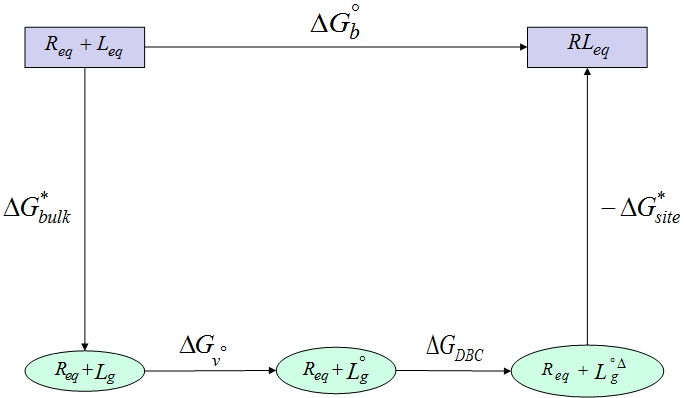
\includegraphics[width=\linewidth]{thermo-cycle}
\caption{The schematic thermodynamic cycle used in the Streamlined AFEP (SAFEP) approach.
$\Delta G_{bind}^\circ$ is the standard free energy of ligand binding to the site.
$\Delta G^*_{bulk}$ is the decoupling free energy of the ligand from the aqueous bulk solvent (minus the excess free energy of solvation).
$\Delta G_V^\circ$ is the free energy of applying the COM restraint on the ligand, with respect to the standard state in gas phase.
$\Delta G_{DBC}$ is the free energy of applying the DBC restraint on the ligand.
$\Delta G^*_{site}$ is the free energy of decoupling the restrained ligand from the binding site.
}
\label{fig:cycle}
\end{figure}

The sum of the free energies for all stages is the absolute binding affinity of the ligand-protein complex:
\begin{equation}\label{eq:delta_G_bind}
    \Delta G_{bind}^\circ = \Delta G^*_{bulk} + \Delta G_V^\circ + \Delta G_{DBC} - \Delta G^*_{site}
   % \label{eq:total_bfe}
\end{equation}

Importantly, note the absence of a stage where restraints are removed in the receptor binding site. This is made unnecessary by the use of well-calibrated flat-bottom potentials on the DBC coordinate and the center of mass, which both have zero impact on the coupled, bound state. This is the major practical benefit of SAFEP.

Of the 4 remaining terms in the right-hand side of Eq.~(\ref{eq:delta_G_bind}), 
two are the results of AFEP decoupling calculations (in bulk water and in the binding site), one ($\Delta G_V^\circ$) has a simple analytical expression ($-RT \ln (V^\mathrm{sphere}/V^\circ)$), and one ($\Delta G_{DBC}$) is estimated by a specific RFEP simulation in vacuum.
That is, the process requires only \textbf{two condensed-phase simulations}, of which one can be done in a small water box.
Importantly, convergence of the AFEP decoupling calculation in the binding site is helped by the DBC restraints, which limits the configurational space that must be sampled.\cite{Salari2018}

In practice, we will determine and apply adequate restraints using the Collective Variables Module\cite{Fiorin2013}, here in its NAMD and VMD versions.
Note that the Gromacs interface could also be used to perform all simulations using Gromacs.



\subsection{Tutorial Overview: Application to the mutant lysozyme-phenol complex}

In this tutorial we will study binding to lysozyme, which has a buried hydrophobic cavity that can trap various small molecules without large conformational changes \cite{Mannhold2012}. To be precise, we will quantify binding of phenol to the L99A/M102H mutated site introduced by Merski et. al. \cite{Merski2013}.
While phenol does not bind significantly to the apolar cavity in wild-type or L99 mutant T4 lysozyme\cite{Deng2006,Wei2002,Morton1995,Graves2005},
it does bind the site created by the L99A/M102H double mutation, with an experimental binding affinity $ \Delta G_{bind}^{o, exp}$ of -5.44~kcal/mol \cite{Merski2013}, to be compared with the result we find for Eq.~(\ref{eq:delta_G_bind}).

% TODO Figure here





\section{Preliminary simulation: exploring the bound state}

In the alchemical decoupling simulation, we decouple the phenol from lysozyme’s binding site to the gas phase while restraining the ligand bound to the bound-state ensemble.
In this alchemical transformation, the ligand’s non-bonded interactions with the environment are progressively decreased to zero.
The flat-bottom DBC restraint should perform two functions:
\begin{itemize}
    \item limit fluctuations of the decoupled ligand as much as possible;
    \item perturb fluctuations of the coupled ligand as little as possible.
\end{itemize}

If we meet the second of these goals, the restraint will leave the bound ensemble unaffected, and therefore have zero free energy contribution to the bound state.
In other words, the DBC-restrained bound state should be essentially the same as the unrestrained bound state.
% A difference is unavoidable somewhere on the edge of the bound state, because in the unrestrained system, the ligand escaping the site may be a rare event, but is always possible. The DBC restraint reduces the tail of the bound-state distribution and makes escape virtually impossible.

% The half-harmonic potential is zero until the DBC reaches a set threshold, at which point a harmonic force kicks in and prevents the ligand from further escaping the bound state (Figure~\ref{fig:scheme-DBC}).
% The boundary value should be set so that most of the bound ensemble is unaffected.
Thus we need a preliminary simulation sampling the bound state to choose the correct DBC boundary value.

Note that such a preliminary simulation is always recommended, whatever the free energy computation scheme, to equilibrate the model of the receptor-ligand complex and characterize it within the chosen modeling parameters (initial structure, force field parameters, solvent model and ionic strength, temperature...).
We may find out that the ligand adopts a different binding pose than expected, say, from an experimental structure of the complex, or perhaps binding is unstable and the ligand escapes the site rapidly.
This should call into question our modeling assumptions, and that is best done before running an expensive AFEP simulation.

\begin{figure}[!ht]
\centering
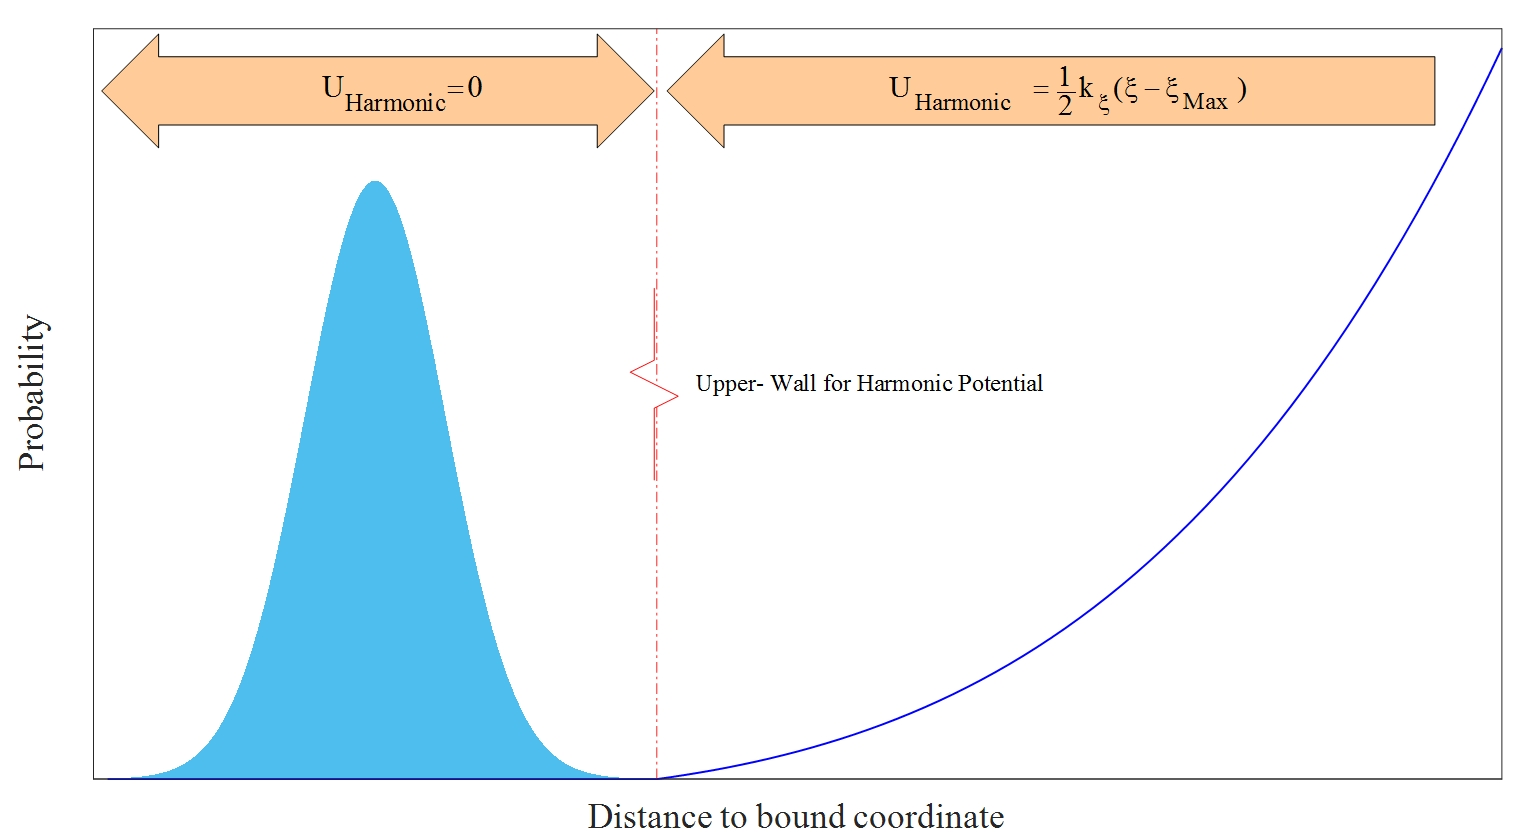
\includegraphics[width=\linewidth]{scheme}
\caption{The schematic representation of the half-well harmonic potential mechanism in the DBC restraint, the blue curve indicates the distance evolution of the half-well harmonic potential.}
\label{fig:scheme-DBC}
\end{figure}

% Below, we describe in detail the procedure to perform the preliminary simulation of the phenol-lysozyme complex.
% As you follow the instructions, you can check the input files provided as Supplementary Information.


\subsection{System preparation }
\label{sec:6.1}

Preparing a protein system for a simulation takes a little work, and is not the focus of this tutorial.
Therefore, we provide the necessary files describing the solvated lysozyme-phenol complex. 
Below, we describe briefly how these files were prepared.

The initial structure of the phenol-mutant lysozyme complex is modeled based on the crystal structure with accession code 4I7L in the PDB.
The structure includes two copies of the complex: we retain only chain A.
We use two tricks to limit the size of the final simulation box:
\begin{enumerate}
    \item We truncate the structure's N- and C-terminal segments that are not tightly associated to the rest of the bundle (residues -11 to 1 and 158 to 164);
    \item We orient lysozyme along the $z$ axis and solvate it in an elongated water box.
Then we need to prevent the protein from rotating during the simulation: we will add a rotational restraint, as explained in section~\ref{sec:rotational restraint}.
\end{enumerate}

We solvate lysozyme in a box of TIP3P water with a physiological NaCl concentration of about 0.15 mol/L.
This can be performed directly in VMD using the psfgen, solvate and ionize plugins (see NAMD tutorial for details\cite{phillips2003}), or using the online tool CHARMM-GUI\cite{Jo2008, Lee2016}.
The initial structure of the solvated ligand-protein complex is rendered in Figure (\ref{fig:assembly}).

\begin{figure}[!ht]
\centering
\includegraphics[width=\linewidth]{lyso5-new}
\caption{Rendering of the solvated lysozyme-phenol complex, with a zoom in the host-guest site. 
}
\label{fig:assembly}
\end{figure}


\subsection{Equilibration}\label{sec:8.2}
\label{sec:equilibration}

\subsubsection{Simulation setup}

The scripts for these simulations are provided as examples.

We use NAMD 2.14\cite{Phillips2020} to minimize, then equilibrate the system at constant temperature of 300~K and constant pressure of 1~bar, controlled by a Langevin thermostat and a Langevin piston algorithm\cite{Phillips2005}.
To prevent anisotropic fluctuations of the periodic cell (preserve its aspect ratio), \texttt{useFlexibleCell} is set to no in the pressure control section.
The periodic boundary condition (PBC) are applied with particle mesh Ewald (PME) long-range electrostatics\cite{Darden1993}, with parameters tailored to the size of the simulation box.
The timestep is set to 2~fs, with constraints on all bonds to hydrogen atoms (\texttt{rigidBonds all}).
The force field is CHARMM36\cite{Best2012}, and the water model is TIP3P\cite{Jorgensen1983}.

The multiple-timestep rRESPA method is used, with fast and slow time steps of 2 and 4 fs, respectively.
\texttt{WrapAll} should be set to \texttt{off}. \texttt{wrapWater} can be set to \texttt{on} optionally.
After the simulation, you can wrap water around the protein in VMD, using the 
% qwrap package (for Linux/MacOS, \url{https://github.com/jhenin/qwrap}) or
PbcTools package.
The center of mass drift of the system is canceled by enabling \texttt{zeroMomentum} and retaining \texttt{COMmotion} at the default value.

The NAMD configuration file also specifies Colvars parameters.
Note that we use "colvar" as shorthand for collective variable, and "Colvars" with a capital "C" for the Collective Variables Module.

Look into \texttt{user\_dir/Supp-File/AFEP-Bound-Decoupling/ equ.namd} configuration file.
In the Colvars section, \texttt{Colvars} is enabled and its input file is specified:
\begin{verbatim}
# COLVARS
Colvars                 on
ColvarsConfig           DBC-unbiased.colvars
\end{verbatim}

This tells the Colvars Module to get its configuration from a file  \texttt{DBC-unbiased.colvars}.
For more information on Colvars configuration, check out the Colvars manual here: \url{ https://colvars.github.io/colvars-refman-namd/colvars-refman-namd.html}\label{clovar}.
% Too detailed for here, just add a comment in the file
% In the colvars script context, using histogram syntax may cause a conflict on NAMD parallel implementation, preventing the "segmentation fault error" followed by this issue, the \texttt{smp} flag is disabled.
% \begin {verbatim}
% smp off
% \end{verbatim}

\subsubsection{Definition of the DBC coordinate}\label{Section 6.2.2}


During the simulation, lysozyme may move frequently altering the binding site atoms conformations. By enabling the \texttt{centerReference} and \texttt{rotateReference} in the rmsd context, the \texttt{fittingGroup} option provides adjusting the phenols’ roto-translational movements to the binding site, the moving reference. In this case, the roto-translational and conformational alterations of phenol are adapted to the proteins' alpha carbons within the 14 {\AA} of phenol.

PDB files can be used for two different roles:
\begin{enumerate}
    \item specify atom groups to use in a collective variable (by setting flags in e.g. the occupancy column);
    \item provide reference coordinates when defining RMSD variables, or variables in moving frames of reference that depend on a fit; the DBC coordinate uses both.
\end{enumerate}

% Some prerequisite files concerning reference atoms such as \texttt{rest-ref.pdb} and \texttt{prot-ref.pdb} are needed to implement the Colvars script. The occupancy value of the reference atoms should be set to 1, creating reference files.
% To prepare the reference pdb files, you can use the sample commands as follows;
% \begin{verbatim}
% #The rest-ref.pdb file contains tagged ligand 
% #and binding site atoms.
% # First reset any non-zero occupancy to zero
% [atomselect top all] set occupancy 0
% # Heavy atoms of phenol
% [atomselect top "resname PHEN and noh"] set occupancy 1
% # Alpha carbons in helices, close to phenol
% [atomselect top "alpha and within 14 of resname PHEN"] \
%     set occupancy 2
% \end{verbatim}

% and in much the same way for the reference of the rotational restraint.
% \begin{verbatim}
% #The carbon alpha atoms in the protein are labeled 
% #in prot-ref.pdb file.
% [atomselect top "alpha and protein"] set occupancy 1
% \end{verbatim}


\begin{verbatim}
# DBC colvar
colvar {
  name DBC
  width 0.1
  lowerboundary 0.0
  upperboundary 5.0
    rmsd {
      # Reference coordinates
      # (for ligand RMSD computation)
      refpositionsfile rest-ref.pdb
      \end{verbatim} 

In the subsequent, we prolong inspecting the rest of commands in the colvars script.
\begin{verbatim}
  atoms {
  # Define ligand atoms used for RMSD calculation
    atomNumbers {11 9 5 1 3 7 12}
\end{verbatim}

Use the serial numbers of objective atoms or molecules to tag accurately in \texttt{atomNumbers} sections. As an example, you can use \texttt{get serial  [atomselect    top    "resname PHEN and noh"]} command in VMD TkConsole, defining phenol as ligand atoms;
\begin{verbatim}
      # Moving frame of reference is defined below
      centerReference yes
      rotateReference yes
      fittingGroup {
        # Define binding site atoms used for fitting
        atomNumbers {32 103 1100 1112 1128 1140 1150
        ...
        2448 2472 2486}
      }
\end{verbatim}

\subsection{Defining the Bound State in Post-processing}
\label{section 6.3}
\begin{enumerate}
\item Run unbiased, vanilla MD of bound state using the configuration files provided:
\begin{verbatim}
user_dir\Supp-Files\DBC-Unbiased\namd2
  equ.namd
\end{verbatim}
then run:
\begin{verbatim}
user_dir\Supp-Files\DBC-Unbiased\namd2
  run.namd
\end{verbatim}
and load the resulting trajectory into VMD. 
\item Choose the protein atoms whose positions define the protein site. In this case, we'll select all alpha carbons that are contacting the bound ligand.   
 \begin{verbatim}
set proteinsel  [atomselect    top "alpha and 
within 14 of resname PHEN"] 
\end{verbatim}
\item Align the trajectory based on these protein atoms, using either the RMSDTT (RMSD Trajectory Tool) GUI in VMD or the command line. 
\item Choose atoms that define the ligand bound state. In this case we'll use all heavy atoms of the ligand: 
\begin{verbatim}
set ligandsel [atomselect top "resname PHEN and
noh"]
\end{verbatim}
\item Calculate RMSD for ligand atoms.
\item Determine your DBC tolerance: the 95th percentile (the value of the RMSD that is higher than 95\% of the equilibrium values) is the lowest DBC tolerance you can use.    
\item Modify DBC colvar in configuration file to specify (a) protein site atoms (b) ligand site atoms (c) DBC tolerance
\end{enumerate}
\subsubsection{Collecting a DBC histogram}\label{section 6.3.1}

We will collect a histogram of the DBC coordinate.
Since we do not know beforehand the relevant range of values, we choose a large enough upper boundary value for all colvars.
We will use the histograms to predict the optimal value of the upper wall for the DBC and center-of-mass (COM) distance variables.

The histogram block makes the data processing simpler and collects data at every time step, although the histogram could be built based on the colvars trajectory file, or even from a posteriori analysis of DCD trajectories using the Colvars Dashboard in VMD.

\begin{verbatim}
histogram {
  colvars DBC
  outputFile DBC.dat
  histogramGrid {
    widths          0.1 
    lowerboundaries 0.0
    upperboundaries 6.0
  }
}
\end{verbatim}

% Tutorial only
\subsubsection{Symmetric DBC}
Phenol rotating around C2 imaginary axis, an axis aligned to the aromatic plane and passing through oxygen, changes the position of carbon atoms in the backbone without conformational transformation.  The free energy contribution of DBC colvar is invariant concerning atom position changes. Accordingly, the \texttt{atomPermutation} keyword is defined to eliminate the impact of the mentioned permutation. Figure (\ref{fig:scheme4}) graphically clarifies the atoms permutation in phenol. It is recommended to use the DBC-symmetry Colvar instead of the conventional DBC Colvar for symmetric and pseudo-symmetric ligands.
\begin{figure}[!ht]
\centering
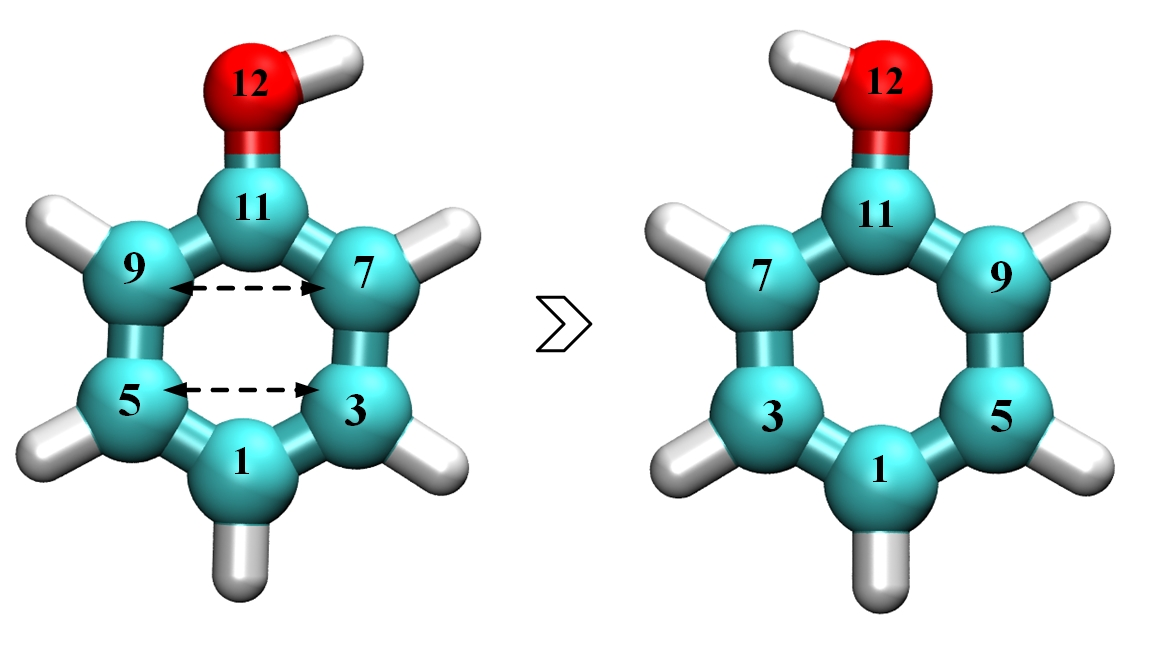
\includegraphics[width=\linewidth]{phenol-permutation-new}
\caption{Four carbon atoms may exchange their positions through phenol rotation without any impact on the conformation of phenol.}
\label{fig:scheme4}
\end{figure}
\begin{verbatim}
# DBC-symmetry Colvar
colvar {
    name DBC_sym
    rmsd {
        atomPermutation {11 7 3 1 5 9 12}
        atoms {
            atomNumbers {11 9 5 1 3 7 12}
\end{verbatim}


\subsubsection{Center-of-mass restraint}\label{section 6.3.3}

The distance colvar reflects the phenol center of mass distance with respect to center of the updated binding site in the protein, moving reference.  A dummy atom with a given coordinate, center of mass of phenol in the bound-configuration, is used to restrain phenol translational movement in the distance colvar.

\begin{verbatim}
# Center of mass distance coordinate Colvar
colvar {
    name distance
    distance {
        group2 { # Reference ligand COM position
            dummyAtom (-2.168, 5.235, 9.367)
# obtained in VMD :
# > measure center [atomselect top "serial 1 3 
5 7 9 11 12"]
\end{verbatim}

\subsubsection{Restraint on protein orientation}\label{sec:rotational restraint}

To keep the water box size at a minimum, lysozyme should be kept aligned along the $z$ axis. By imposing a harmonic force on rotation components, we preserve the initial orientation of lysozyme. Hence, the \texttt{closestToQuaternion} keyword is set to identity rotation. The rotation act is expressed in quaternion, a four-dimensional vector (q$_1$, q$_2$, q$_3$, q$_4$), furnishing \( \sum_{i}q_i^2=1\) \cite{Bar-Itzhack2000,Eberly2002}. As quaternion components have a magnitude less than 1, so a high enough harmonic bias force constant is required, providing the unit quaternion.
\begin{verbatim}
 colvar {
    name rotation
    orientation {
       # Reference coordinates (for protein)
       refpositionsfile prot-ref.pdb 
       atoms {
       # Define protein atoms used for optimal rotation
       atomNumbers {18 32 51 71 86 103 122 146 165 177 
       .... 2493}
        }
       # Define reference rotation to null orientation
       closestToQuaternion (1.0, 0.0, 0.0, 0.0)
    }
 }
# Harmonic restraint on rotation       
 harmonic {
    colvars       rotation
    forceConstant 10000.0
    centers       (1.0, 0.0, 0.0, 0.0)
 }
\end{verbatim}

\subsection{Production run}\label{section 6.4}
After completing the short equilibration, the production simulation is carried out starting from equilibration restart files. The configuration file for the production run is the same as the equilibration, only the set value for \texttt{margin} keyword should be removed. The \texttt{margin} parameter extends the system in all dimensions avoiding the "patch grid error" at the beginning of the simulation. So, if you did not face this error, you can jump over the equilibration step in the unbiased simulation. Furthermore, the production run is executed long enough to collect an ensemble describing the fluctuations of the bound state.
\begin{verbatim}
user_dir\Supp-Files\DBC-Unbiased\namd2  run.namd
\end{verbatim}
% At the start point of the equilibration, expansion of the system occurs since the initial structure is constructed manually. In this undesired incident, the margin parameter considers extra lengths in system dimensions avoiding the patch grid error. i.e. “FATAL ERROR: Periodic cell has become too small for original patch grid”. For achieving more reliable performance, the margin keyword is set to the default value again in the production run.

\subsection{Result assessment}

Inspect the trajectory visually in VMD and examine the binding mode of the ligand, its motion with respect to the protein, and its interactions with  protein residues.
Plot the histogram for the DBC and distance variables to decide the best maximum value for the flat-bottom harmonic restraint.
Using the Colvars Dashboard, plot these variables along the trajectory to interpret each peak in their distribution in terms of phenol's position and interactions with the protein.

% Therefore, execute the command line below in your histogram outputs directory. You will find the same result by assessing the trajectory output file. Notice that you may learn more about the python script and requirements in its’ official website \url{https://www.python.org}. In the directory of the histogram results, type in the  command as the same as below. Histograms in Figure (\ref{fig:DBC-histogram}) are obtained by colvars outputs.
% \begin{verbatim}
% ..\Plot-histogram.py  DBC.dat  DBC-Symmetry.dat COM-Distance.dat
% \end{verbatim}


% \begin{figure}[h!]
% \centering
% 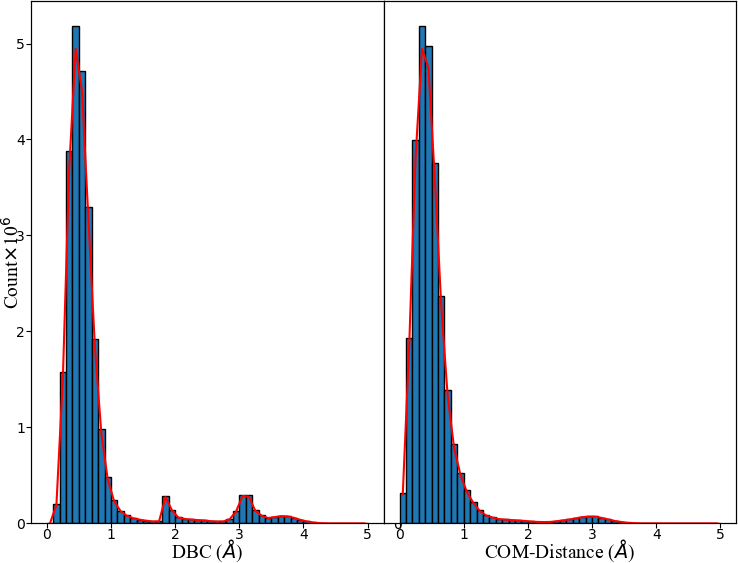
\includegraphics[width=\linewidth]{histogram_nosym}
% \caption{DBC and DBC-Symmetry histograms display the distribution of phenol distance from bound-configuration. Similarly, the COM-Distance histogram represents the spread of the distance between phenol and center of mass of coupled-configuration relative to the moving reference.}
% \label{fig:DBC-histogram}
% \end{figure}

% The emerged sharp peak in Figure (\ref{fig:DBC-histogram}) signifies a predominant phenol orientation in the configuration state, multiple peaks with fewer occurrences attributed to unstable conformations. In the DBC histogram, peaks may indicate different conformations of the coupled phenol that its’ structural alterations and the trajectory timeline need scrutinizing via \texttt{colvars} dashboard in the VMD. In Figure (\ref{fig:DBC-histogram}), the second peak around 2 {\AA} with small height is entirely disappeared in the DBC-Symmetry histogram, achieved by using atom permutation feature in the colvars input. The rotation of phenol around its’ C{$_2$} imaginary-axis brings about two indistinguishable bound-configurations. Since these two conformations induced by symmetrical rotation function are the same in the binding site, the atom permutations syntax is defined to eliminate the influence of conformational alterations in the free energy assessment. By inspecting the histogram result, we assume the harmonic bias upper-wall where the curvature starts decaying to zero. Non-bonding interactions and hydrogen bonds influence the orientation of phenol in the coupled-configuration state. The study of the trajectory timeline and visual data confirms that the hydroxyl of phenol mainly forms a H-bond to the imidazole cycle in the histidine residue in the binding pocket. Although the H-bond between phenol and leucine residue is also observed inside the binding site, the small peak appeared about 3 {\AA} in Figure (\ref{fig:DBC-histogram}), the contribution of this unstable conformation is trivial enough to be neglected. Accordingly, 1.5 {\AA} is a reliable estimation for the harmonic bias upper-wall in the AFEP simulation. Figure (\ref{fig:snapshot}) delineates H-bond between phenol and histidine or leucine residues in the binding cavity. It is worthy to note that the upper-boundary of the harmonic restraint could be measured using a normalized cumulative frequency analysis as well, and the upper-wall value is accurate when the cumulative frequency is over 0.9.

\begin{figure}[h!]
\centering
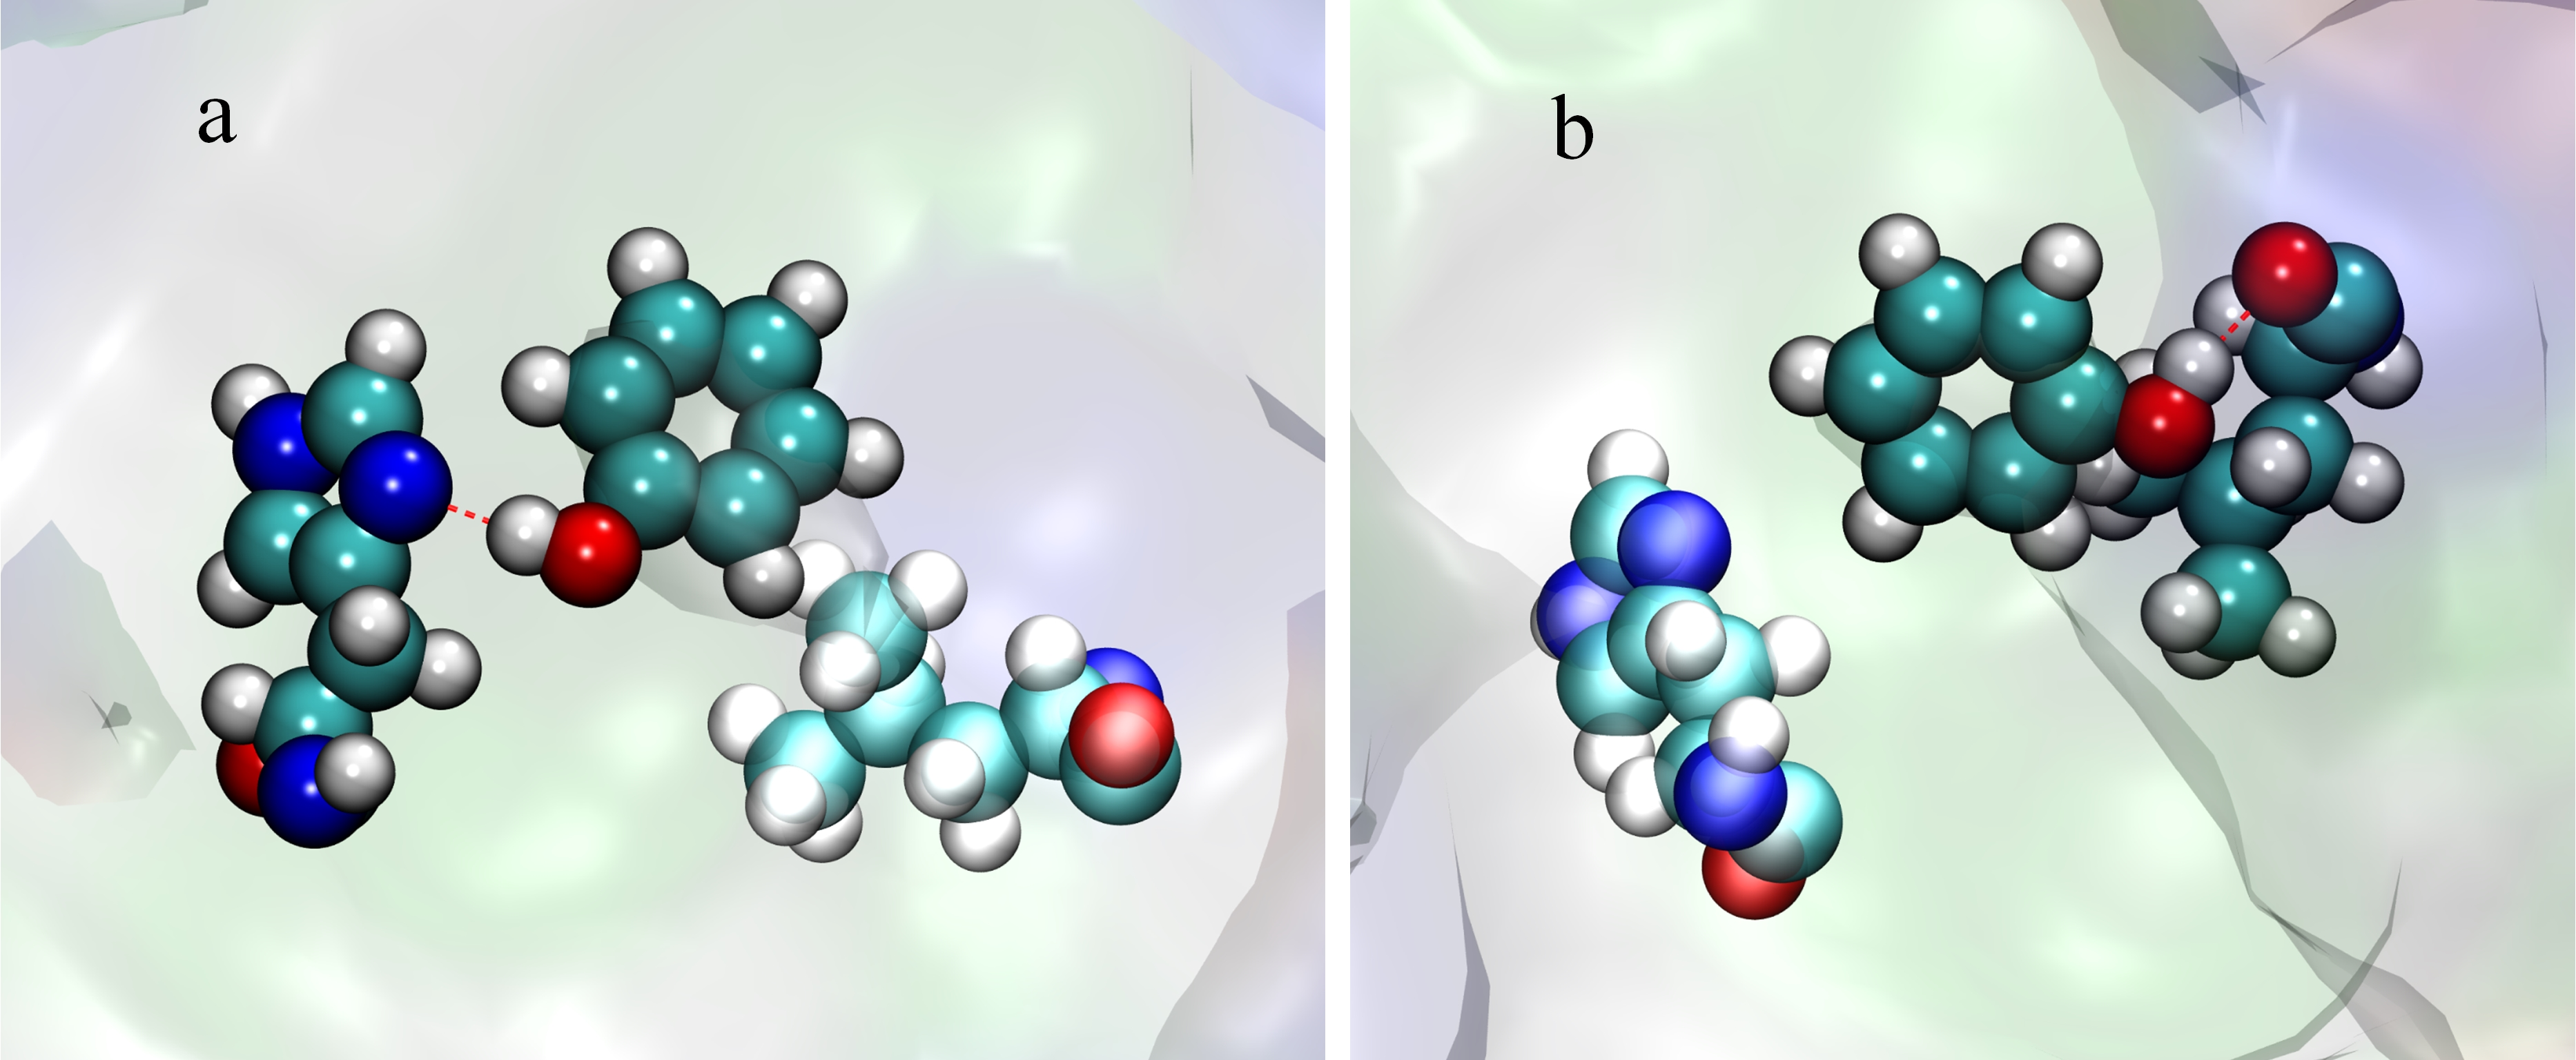
\includegraphics[width=\linewidth]{HSELEU}
\caption{Two detected bound configurations for phenol in the binding pocket. In the snapshots phenol forms a hydrogen-bond with (a) a histidine and (b) a leucine residue.}
\label{fig:snapshot}
\end{figure}

% When the estimation with high accuracy is required instead of ignoring the unstable coupled-conformation, you can re-run the simulation with the emerged conformation as initial structures and new reference files, considering the contribution of this calculated free energy to the overall estimation. Therefore, all bound-conformations are engaged in free energy calculation. We did not apply this procedure in this tutorial, and we skipped the insignificant conformation, which the related peak appeared around 3 {\AA}.

\section{Decoupling the ligand from the binding site}\label{section 7}

\subsection{Simulation under DBC restraint}\label{section 7.1}

% Preliminary equilibration of the lysozyme-phenol complex under the DBC restraint is necessary.
% \jh{If the DBC upper wall is well-chosen, the system equilibrated without restraint can be directly simulated with the restraint, because the restraint should be neutral. So this equilibration can be quite short. The most important info in this subsection is the definition of restraints. I changed the title accordingly.}

It may require a long enough equilibration simulation until the Rmsd of lysozyme behaves time independent below 3 {\AA}. Furthermore, the smooth time evolution of DBC colvar trajectories could be another evidence of the equilibration. We use the \texttt{equ.namd} configuration file the same as the \texttt{run.namd} file without any modification for this section. In the colvar input file, the measured maximum DBC from the previous subsection (unbiased simulation) should be replaced with the values for \texttt{upperboundary} in DBC colvar and histogram blocks. we also utilize this DBC maximum value as the upper wall of the harmonic restraint to implement harmonic bias outside of this range. For applying DBC restraint on the coupled complex, we only added harmonic restraint components to the colvar input script. New keywords in the \texttt{DBC-Restraint.colvars} input file are presented in the following:
\begin{verbatim}
#   Flat-bottom harmonic restraint on DBC 
harmonicWalls {
colvars           DBC_sym
upperWalls        1.5
forceConstant     200
}
\end{verbatim}

\subsection{Production run}

The fep file format is required to introduce outgoing and incoming atoms for the AFEP evaluation. In this case, the phenol is annihilated in the binding site and the rest of the system is remained without alterations, so beta-column for the phenol should be set to -1 in the fep file format. The \texttt{fep.tcl} script enclosed as supplementary Files is required for the alchemical free energy (AFEP) calculations.
%You can Create the fep file by using the \texttt{fep.tcl} script enclosed as supplementary information.

To perform the AFEP run, we start from the equilibration restart files with the same conventional MD simulation details discussed before in the unbiased simulation. Now we have a look into the \texttt{run.namd} file in the "AFEP-Bound-Decoupling" folder to define sampling strategy for the alchemical simulation.
\begin{verbatim}
# FEP PARAMETERS
source               ./fep.tcl
alch                 on
alchType             FEP
alchFile             solv-prot-charmm.fep
alchCol              B
alchOutFreq          2
alchOutFile          AFEP2-02.fepout
\end{verbatim}
The accurate estimation of free energy differences ($\Delta F$) provided by BAR or SOS methods is highly dependent on a sufficiently large number of samples. Hence, the \texttt{alchOutFreq} should be assigned small enough to improve the evaluation of the free energy differences by decreasing error bars. It is recommended to define \texttt{alchOutFreq} as either 1 or a multiple of \texttt{fullElectFreq}. For more information, please check the \href{https://www.ks.uiuc.edu/Research/namd/mailing_list/namd-l.2020-2021/1487.html}{Bug advisory and Workaround}.
\begin{verbatim}
alchElecLambdaStart   0.5
alchVdwLambdaEnd      1.0
alchVdwShiftCoeff     5.0
\end{verbatim}
soft-core potential parameters are utilized to prevent the “end-point catastrophe” by gradual scaling of nonbonded interactions of disappearing atoms with the environment. In this case, the default values fulfill aimed results properly.
\begin{verbatim}
alchdecouple          on
\end{verbatim}
By setting the \texttt{alchdecouple} keyword on, in the alchemical transformation, the interatomic nonbonded interactions of changing atoms are not contributed to the free energy estimation.
\begin{verbatim}
alchEquilSteps  500
set  numSteps   50000
set  dLambda    0.05
runFEP    0.0   1.0  $dLambda   $numSteps    true
\end{verbatim}
The alchemical FEP sampling is performed by 20 windows with equal intervals i.e. {$\Delta\lambda$=0.05}, each window is run for 50000 steps interleaved with 500 equilibration steps.
The true value at the end of \texttt{runFEP} command enables interleaved double-wide sampling (IDWS), as a result of the utilization of this feature, the forward and backward free energy calculation is performed concomitantly. The IDWS provides a fast and an accurate estimation by the frequent interchange of {$\lambda$} between forward and backward values. If the \texttt{alchLambdaIDWS} keyword is defined by denoting a given value, the backward free energy will be estimated in the certain range of {$\lambda$}.

\subsection{Result assessment}
The AFEP simulation output can be analyzed with either the VMD or the alchemlyb library to assess the free energy result. The interleaved double-wide sampling (IDWS) interlaces forward and backward data in the output file, which is extracted by post-processing the fepout file. We compressed folders possessing large output files with tar command in the subdirectories of \texttt{/Supp-Files/} (provided as supplementary files). To follow the tutorial in the Result section, you need extracting tar files, navigate linux or MacOS terminal to the directory of tar files and use the following command:
\begin{verbatim}
tar -xzvf name.tar.gz
\end{verbatim}
In Windows, you can also extract tar files by opening them with WinZip and clicking Unzip.
\subsubsection{Ligand binding free energy: ParseFEP plugin in VMD}
Before performing the FEP analysis with ParseFEP plugin \cite{Liu2012} with VMD, a python script is used to deinterlace the forward and backward data. Execute the deinterleave-idws.py file by the subsequent command.
\begin{verbatim}
user_dir/Supp-Files/AFEP-Bound-Decoupling/output/
VMD-ParseFEP/python  deinterleave-idws.py
  ../AFEP2-02.fepout
\end{verbatim}
Following the execution of the Python script, two output files, \texttt{AFEP2-02\_bwd.fepout} and \texttt{AFEP2-02\_fwd.fepout}, are generated in the \texttt{VMD-ParseFEP} folder, representing backward and forward free energy change from sampling of each window. The VMD 1.9.4 is needed to proceed with the free energy estimation, using the ParseFEP plugin \cite{Liu2012}.
In the main menu of VMD, click the \texttt{Extensions} and from the drop down menu, select \texttt{Analysis} and then \texttt{Analyze FEP Simulation} to open the \texttt{ParseFEP} plugin. In the parameter section of the \texttt{ParseFEP} plugin, set the \texttt{Gram-Charlier order} to zero and enable pictorial representation by checking the \texttt{disp} option. The forward and the backward outfep files are chosen as FEP and FEP (backward) output files and \texttt{run FEP Parsing}, employing the \texttt{BAR estimator}. The ParseFEP graphical interface provides free energy estimation combining forward and backward results with the help of the \texttt{SOS} or the \texttt{BAR estimator}. 
%In Figure (\ref{fig:AFEP-decoupling1}), you can find phenol free energy results, decoupling from the binding site environment.

%\begin{figure}[th!]
%\centering
%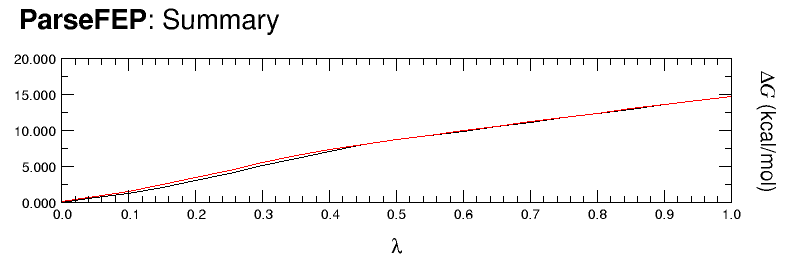
\includegraphics[width=\linewidth]{AFEP-decoupling-sum}
%\caption{The {$\lambda$}-evolution of the forward and the backward phenol decoupling free energy, from the lysozyme binding site, is evaluated using the ParseFEP plugin in VMD.}\label{fig:AFEP-decoupling1}
%\end{figure}
\subsubsection{Ligand binding free energy: Alchemlyb library}
An alternative to the AFEP calculation is the alchemlyb library that recently supports the NAMD's IDWS feature \cite{chodera2016simple, shirts2008statistically}, providing the BAR and the MBAR estimators. A jupyter notebook documented by \href{https://github.com/BranniganLab/safep}{Dr. Grace Brannigan's Lab}, /Supp-Files/Jupyter-notebook/BAR\_NAMD\_alchemlyb.ipynb, conveniently sets up a broad series of built-in functions and tools of the alchemlyb library in a straightforward framework, including parsing the fepout file, AFEP calculation, as well as qualitatively comparing the free energy results in different plot types. Launch a jupyter notebook in the directory of \texttt{BAR\_NAMD\_alchemlyb.ipynb} file:
\begin{verbatim}
user_dir/Supp-Files/AFEP-Bound-Decoupling/output/
Alchemlyb/jupyter notebook
\end{verbatim}
In the tree view of the jupyter notebook interface, click the \texttt{BAR\_NAMD\_alchemlyb.ipynb}. In Figure (\ref{fig:BAR_NAMD_alchemlyb}), the snapshot of the first cell in the the \texttt{BAR\_NAMD\_alchemlyb.ipynb} is rendered. Replace the texts in the blue and yellow highlighted boxes with the fepout filename and path. To analyze the fepout file, click the \texttt{Cell} in the top navigation bar of the jupyter notebook and then select the \texttt{Run All}. 
\begin{figure}[h!]
\centering
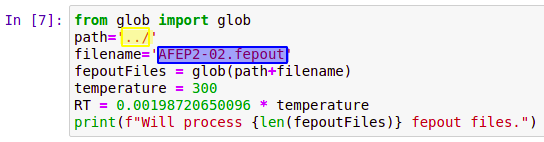
\includegraphics[width=\linewidth]{ipynb.png}
\caption{The rendering of the first cell in the \texttt{BAR\_NAMD\_alchemlyb.ipynb} jupyter notebook.}\label{fig:BAR_NAMD_alchemlyb}
\end{figure}

For the forward and reverse sampling, the alchemlyb library uses the Bennett acceptance ratio (BAR) estimator to calculate the difference free energy for each window and estimate the overall free energy at {$\lambda$}=1 by ensemble averaging over all {$\lambda$}-windows. Correspondingly, the evolution of the phenol binding free energy relative to {$\lambda$} is obtained from parsing the \texttt{AFEP2-02.fepout} with the jupyter notebook and illustrated in Figure (\ref{fig:AFEP-decoupling1}). According to Figure (\ref{fig:AFEP-decoupling1}) and the screenshot of the printed data in the notebook represented in Figure (\ref{fig:ipynb-cell4}), the phenol decoupling affinity from the binding site is estimated at about (14.65$\pm$0.38) kcal/mol.

\begin{figure}[th!]
\centering
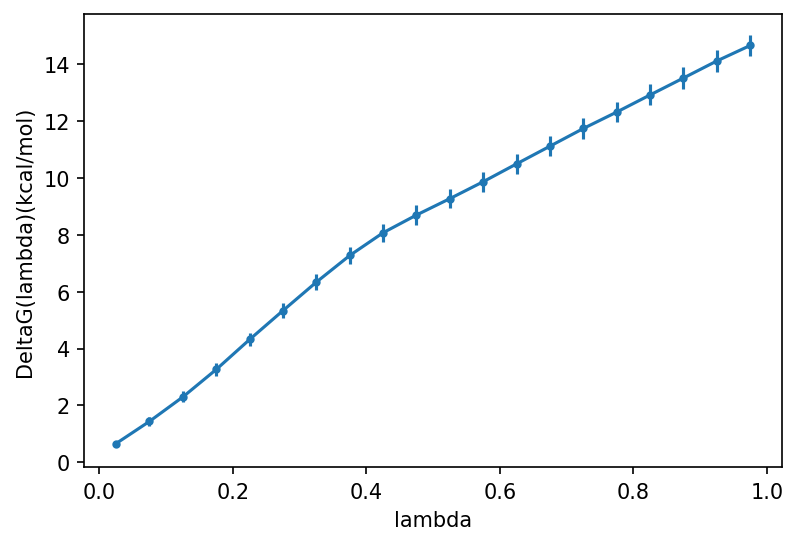
\includegraphics[width=0.8\linewidth]{Supp-Files/AFEP-Bound-Decoupling/output/Alchemlyb/output_4_1.png}
\caption{The {$\lambda$}-evolution of the phenol decoupling free energy, from the lysozyme binding site, evaluated by the Alchemlyb library.}\label{fig:AFEP-decoupling1}
\end{figure}

\begin{figure}[h!]
\centering
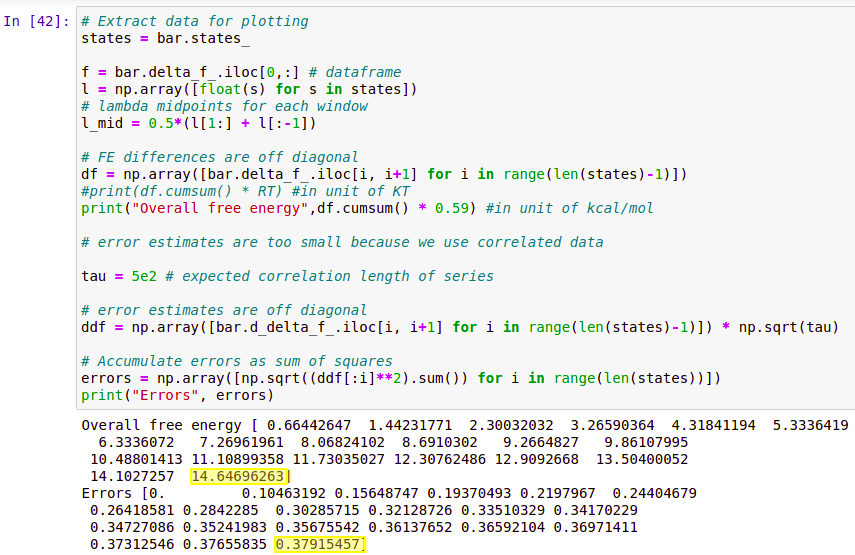
\includegraphics[width=0.9\linewidth]{ipynb-cell4.png}
\caption{The rendering of a patch of the \texttt{BAR\_NAMD\_alchemlyb.ipynb} notebook. The free energy data with statistical errors for each window is printed in two separate arrays.}\label{fig:ipynb-cell4}
\end{figure}
The time evolution of phenol decoupling affinity from the binding site for forward sampling and the reverse is well converged in Figure (\ref{fig:AFEP-decoupl2}). Figure (\ref{fig:AFEP-decoupl2}), for example, compares the free energy in the first and the last 10{$\%$} of the sampling, collecting data from the forward pathway and the reverse, and extending the sampled data to the total as the fraction of time increases. The convergence of the forward and reverse sampling is crucial to optimize the AFEP simulation benefiting from efficient and affordable simulations. The maximum overlap in the free energy estimated from the forward and backward sampling leads to fast convergence. As well as the ParseFEP plugin, the alchemlyb library visualizes the convergence and discrepancy of the forward and backward difference free energy. For decoupling phenol from the bound-state, the forward and backward discrepancy in the binding affinity with respect to {$\lambda$} and its' distribution over the difference free energy are illustrated in Figure (\ref{fig:AFEP-decoupl3}).

\begin{figure}[h!t]
\centering
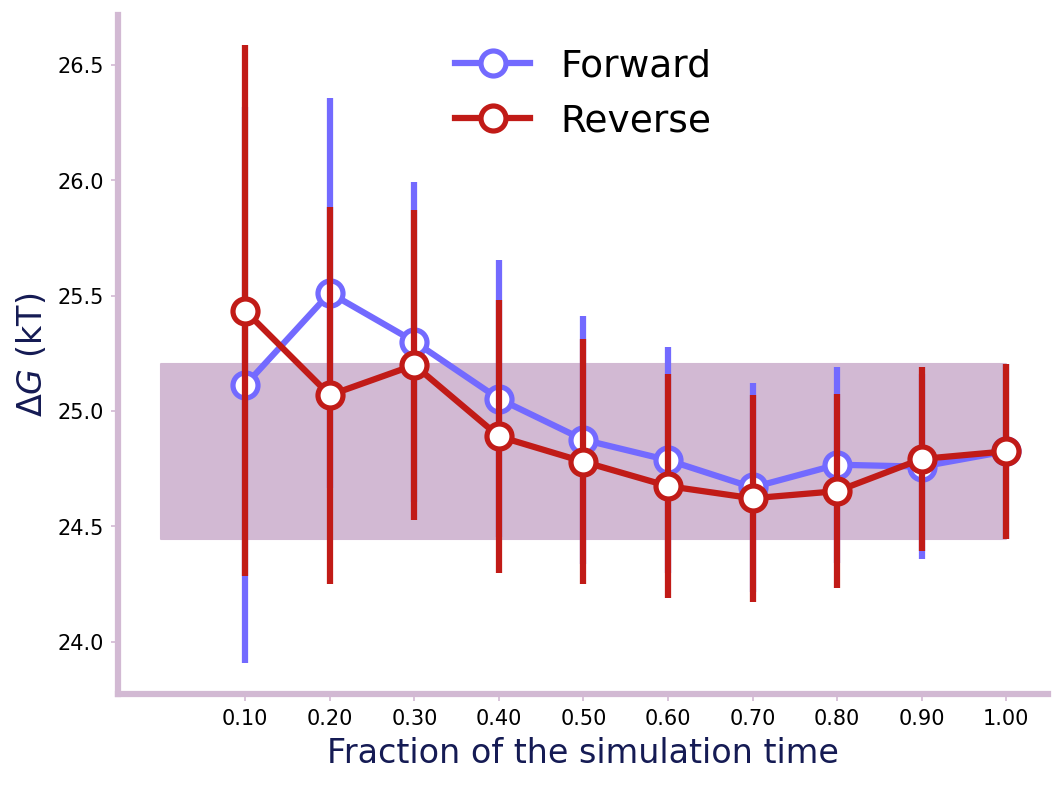
\includegraphics[width=0.85\linewidth]{Supp-Files/AFEP-Bound-Decoupling/output/Alchemlyb/output_5_0.png}
\caption{The convergence of the free energy of phenol decoupling from the binding site in the given fractions of simulation time is represented for the forward and backward transformations.}
\label{fig:AFEP-decoupl2}
\end{figure}

AFEP simulations with appropriate {$\lambda$} intervals, number of sampling, and, in particular, soft-core potential parameters are expected to either exhibit small fwd-bwd affinity discrepancies over the last {$\lambda$}s or, in other words, to exhibit a unimodal distribution of fwd-bwd free energy discrepancies around zero.

\begin{figure}[h!t]
\centering
(a)
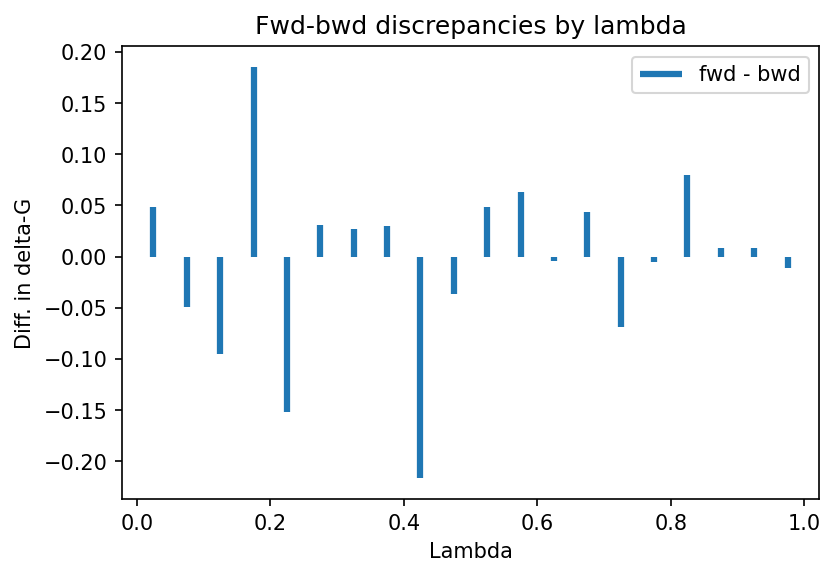
\includegraphics[width=0.8\linewidth]{Supp-Files/AFEP-Bound-Decoupling/output/Alchemlyb/output_7_1.png}
\\
\centering
(b)
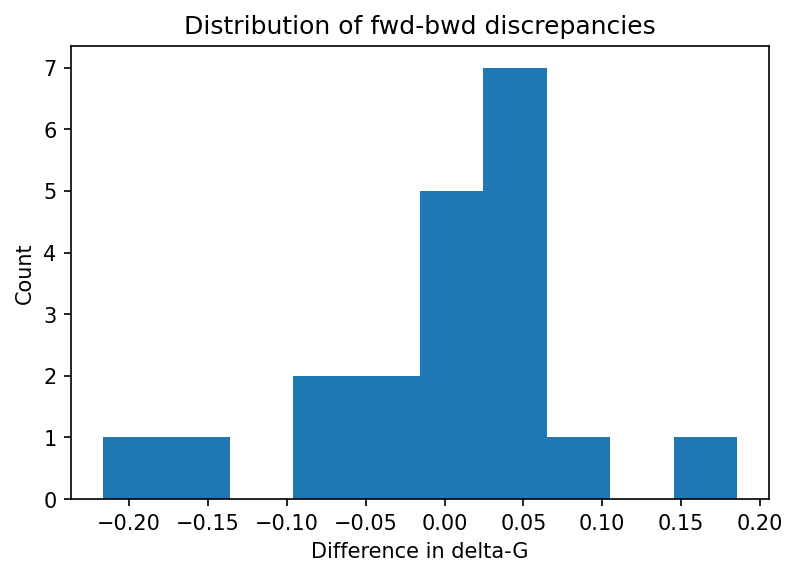
\includegraphics[width=0.8\linewidth]{Supp-Files/AFEP-Bound-Decoupling/output/Alchemlyb/output_8_1.png}
\caption{ For decoupling phenol from the binding site (a) shows the forward-backward free energy discrepancy relative to {$\lambda$} and (b) represents the distribution of the fwd-bwd binding affinity discrepancy.}
\label{fig:AFEP-decoupl3}
\end{figure}

\section{Restraint free energy calculation}\label{sec:10}
Imposing bias potentials on degrees of freedom of the ligand definitely affects the sampled statistical distribution,leading systematic error in the estimation of absolute binding free energy. To remedy this, we calculate restraint energies and consider their contributions to the overall free energy \cite{Henin2014,Fu2017}.

\subsection{Distance from bound-configuration restraint}
Although gradual removal of the DBC restraint helps the phenol to retain the bound-conformation during decoupling, the contribution of the DBC restraint must be deducted from the overall free energy estimation. A common approach to handle this issue is establishing the DBC restraint on the phenol progressively, whereas it is confined in an enclosed volume. Employing the harmonic bias with changing force constant in the Colvars module allows us to launch the DBC restraint on the phenol step by step in the RFEP simulation.

\subsection{Implementation of the RFEP simulation}\label{section 8.2}
The molecular dynamics simulation of the volume enclosed phenol under DBC restraint is practiced through a conventional NVT MD at the constant temperature of about 300 k, controlled by Langevin thermostat. In the configuration file, both the \texttt{PME} and the \texttt{cell basis vectors} as subcommands of the PBC are disabled. The \texttt{wrapWater} and the \texttt{wrapAll} keywords are set to off, followed by disabling the PBC. Here, we investigate the colvars input, \texttt{DBC-Restraint-RFEP.colvars}, and utilized commands for executing RFEP simulation. All keywords used to tailor the phenol roto-translational and conformational changes to the moving reference, including fittingGroup block, are omitted in the colvar context, because the phenol is confined within a discrete volume in the absence of the receptor. In this regard, the \texttt{centerReference} and the \texttt{rotateReference} options are set to off because we do not need defining the optimal ligand roto-translational alignment upon the bound-configuration. To enclose the phenol inside the determined volume, a harmonic bias must be put on the distance colvar during the whole simulation time.

The RFEP output data files are assessed using the thermodynamic integrating method. We introduce a harmonic bias with the force constant evolving nonlinearly relative to {$\lambda$}, avoiding singularity or integration problems. Thus, it would be sensible to set the value of the \texttt{targetForceExponent} higher than 1, chosen by trial and error for this system. Intending to apply the DBC restraint progressively, the force constant of the bias potential starts from zero and increases as a function of the coupling parameter to provide the target force constant.

\begin{verbatim}
# Changing flat-bottom harmonic restraint on DBC 
harmonicWalls {
    colvars               DBC_sym
    targetForceConstant   200.0
    targetForceExponent   6.0
    upperWalls            1.5  
    forceConstant         0.0
    targetEquilSteps      500
    lambdaSchedule        1.00 0.95 .... 0.05 0.00
    targetNumSteps        500000
}
\end{verbatim}

The RFEP simulation is performed using an arbitrary series of \texttt{lambdaSchedule} with a specific interval ({$\Delta\lambda$}) of about 0.05. Each window of the desired \texttt{lambdaSchedule} is sampled over \texttt{targetNumSteps} steps with \texttt{targetEquilSteps} prior equilibration steps.


\subsection{Result assessment}
The RFEP simulation does not generate any individual output file reflecting the calculated free energy. We need to extract the primary data from the general NAMD log file (\texttt{rfep.log}), written in front of colvars rows with \texttt{dA/dLambda} notation. To have a clear vision, a cut of colvars rows in the \texttt{rfep.log} file is displayed in Figure (\ref{fig:RFEP1}). 

\begin{figure}[h!t]
\centering
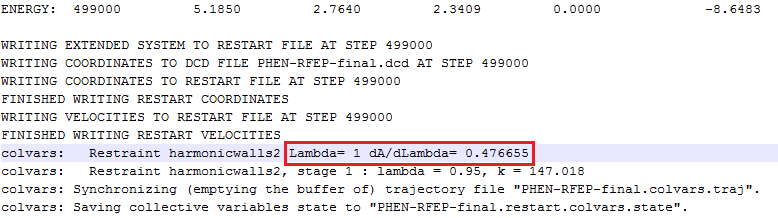
\includegraphics[width=\linewidth]{RFEP-log}
\caption{A sample cut of the \texttt{rfep.log} file by highlighting the primary data for restraint free energy calculation. }
\label{fig:RFEP1}
\end{figure}

The derivative of free energy as a function of {$\lambda$} (\texttt{dA/dLambda}) are collected from the NAMD log file by Using the following Unix command and saving to the \texttt{RFEP.dat} file.
\begin{verbatim}
grep "Lambda="  rfep.log | awk '{print $5, $7}' >
 RFEP.dat
\end{verbatim}

In the former subsection, the implementation of the RFEP simulation, the restraint free energy was defined using a non-linear changing harmonic potential with respect to the coupling parameter ({$\lambda$}). Here, we estimate the restraint free energy difference between the reference and the target states through the integral of the free energy derivative over the {$\lambda$}, referred to as the thermodynamics integrating method \cite{Kirkwood1935,frenkel2001understanding}. Eventually, the RFEP free energy is obtained, using \texttt{xmgrace} for integrating the \texttt{dA/d$\lambda$}, by typing \texttt{xmgrace rfep.dat} command in the Unix terminal, and selecting \texttt{cumulative sum} from \texttt{Data  {$\rightarrow$} transformation {$\rightarrow$} Integration} on the top navigation bar. The \texttt{dA/d{$\lambda$}} and its’ integrating relative to the {$\lambda$} is illustrated in Figure (\ref{fig:RFEP2}). The restraint free energy is measured of about -1.97 kcal/mol by employing the thermodynamic integration method. 
\begin{figure}[h!t]
\centering
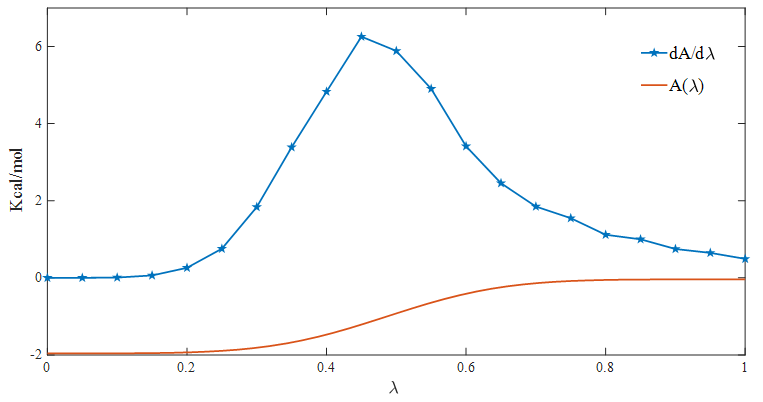
\includegraphics[width=\linewidth]{RFEP}
\caption{Restraint free energy ($A(\lambda)$, red line) and its derivative with respect to the coupling parameter ($dA/d\lambda$, blue line), as a function of {$\lambda$}.}
\label{fig:RFEP2}
\end{figure}

\subsection{Isotropic center-of-mass restraint}
The DBC restraint was released while restraining the center of mass of phenol to a spherical enclosing volume. In the next stage, the geometry confined phenol is exchanged between the isotropic and the anisotropic, consistent with the bulk, interaction environments. The free energy cost of this transmission between two environments relies on the ratio of their volumes, which can be calculated by Eq.~(\ref{equ6}).
\begin{equation}\label{equ6}
\Delta F_{iso}=-RT\ln{\frac{V_{bulk}}{V_{confined}}}
\end{equation}

The {$V_{confined}$} , geometry confined, is obtained by {$\frac{4}{3}\pi r^{3}$} and r is the upper boundary of the applied harmonic bias on the distance colvar. The {$V_{bulk}$} notation displays the volume of bulk with standard concentration \cite{Salari2018}. According to Eqn(\ref{eq:delta_G_bind}), the contribution of the switch to the isotropic restraint in the overall free energy is calculated about 2.84 kcal/mol.

\section{Decoupling the ligand from bulk solution}\label{sec:11}

In this section, phenol is decoupled from the solution in the absence of lysozyme. We calculate the free energy of phenol decoupling from solution based on the alchemical free energy method, using the Bennett acceptance ratio (BAR) estimator for better convergence. Accordingly, the same sampling framework used in decoupling phenol from lysozyme is applied with a little modification. The time step of 1 fs is chosen for the solvated phenol, in view of the fact that the small size of the system satisfies a cheap simulation. The \texttt{Colvars} block is disabled in the configuration file as the phenol is not restrained in the solution. In decoupling phenol from the solution, the value of \texttt{alchVdwShiftCoeff} is set to 6.8 in the soft-core potential parameters. 

\begin{verbatim}
alchVdwShiftCoeff     6.8
\end{verbatim}

\begin{verbatim}
alchEquilSteps        50000
set  numSteps         450000
set  dLambda          0.05
runFEP   0.0   1.0  $dLambda   $numSteps  true
\end{verbatim}
The alchemical FEP sampling for decoupling phenol from the solution is performed by 20 windows with equal intervals i.e. {$\Delta\lambda$=0.05}, each window is run for 450000 steps interleaved with 50000 equilibration steps. In this case, the equilibration steps and number steps for each window are increased.

\subsection{Result assessment}
We analyze the AFEP simulation output by alchemlyb library through the procedure as mentioned earlier. The free energy difference of the ligand decoupling from aqueous solution is measured of about (4.18{$\pm$}0.21) kcal/mol and its’ evolution with respect to {$\lambda$} is illustrated in Figure(\ref{fig:AFEP-Hyd-1}).
\begin{figure}[h!t]
\centering
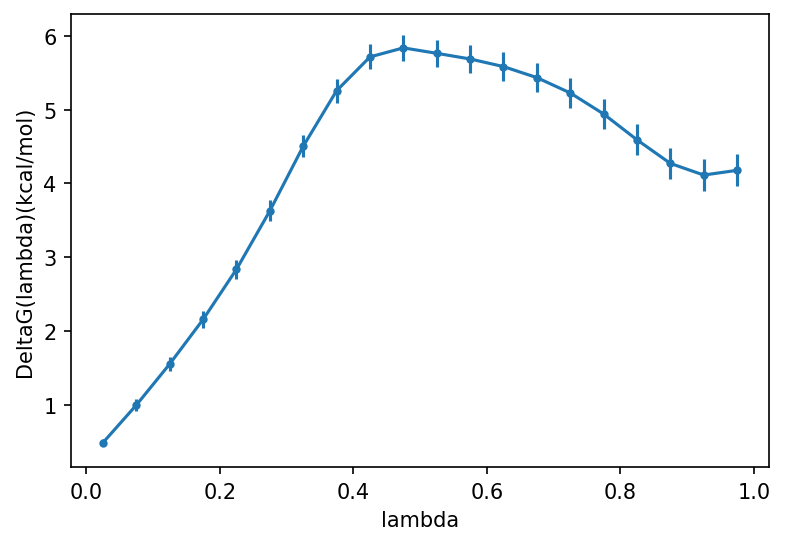
\includegraphics[width=0.9\linewidth]{Supp-Files/AFEP-Hydration/output/Alchemlyb/output_4_1.png}
\caption{The {$\lambda$}-evolution of phenol decoupling affinity, from aqueous bulk solution, evaluated using alchemlyb library.}
\label{fig:AFEP-Hyd-1}
\end{figure}

To put the convergence analysis on the phenol decoupling free energy from the aqueous solution or called phenol hydration affinity, we provided Figure (\ref{fig:AFEP-Hyd-1}) visualizing the time-evolution of the forward and reverse sampling. Similar to the ligand binding free energy section, you might find the forward and backward discrepancy of phenol hydration affinity changing with {$\lambda$} and its' distribution over the free energy in Figure (\ref{fig:AFEP-Hyd-2}).

\begin{figure}[h!t]
\centering
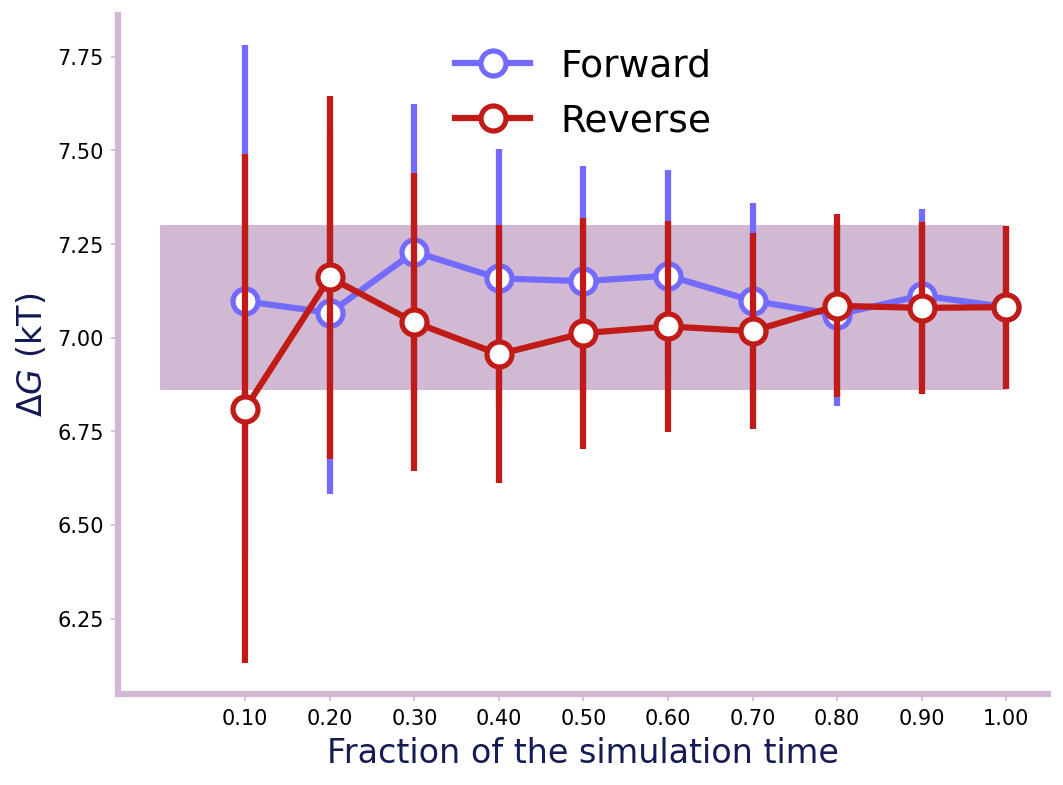
\includegraphics[width=0.9\linewidth]{Supp-Files/AFEP-Hydration/output/Alchemlyb/output_5_0.png}
\caption{The phenol hydration affinity estimated from the forward and backward sampling changes as a function of fractions of simulation time.}
\label{fig:AFEP-Hyd-1}
\end{figure}

The small fwd-bwd discrepancy of phenol hydration affinity may indicate the negligible hysteresis between the forward pathway and the reverse, which enhances the accuracy of the estimation.

\begin{figure}[h!t]
\centering
(a)
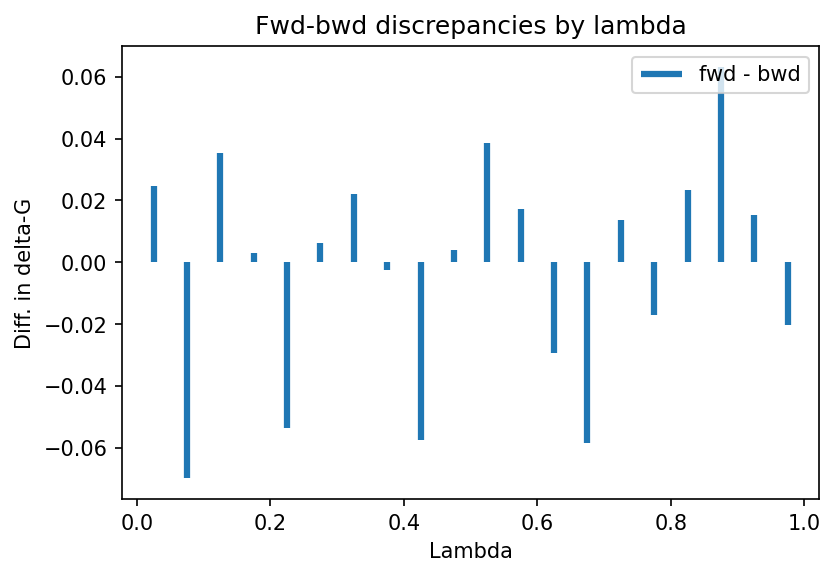
\includegraphics[width=0.8\linewidth]{Supp-Files/AFEP-Hydration/output/Alchemlyb/output_7_1.png}
\\
\centering
(b)
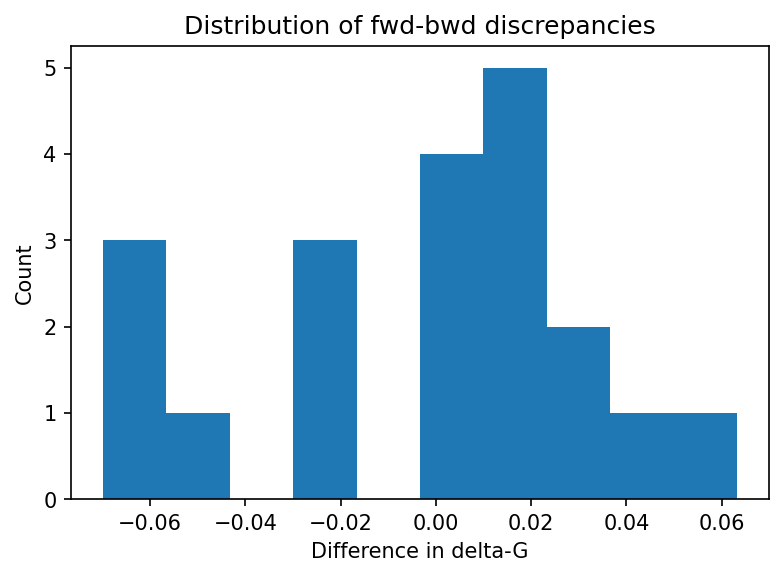
\includegraphics[width=0.8\linewidth]{Supp-Files/AFEP-Hydration/output/Alchemlyb/output_8_1.png}
\caption{(a) The fwd-bwd discrepancy of the phenol hydration free energy over $\lambda$ window, and (b) the distribution of the fwd-bwd discrepancy of the phenol hydration affinity. }
\label{fig:AFEP-Hyd-2}
\end{figure}


\section{Calculating the absolute binding free energy}\label{sec:12}

Ultimately, all obtained free energies for non-physical intermediate states are added up to estimate the absolute binding free energy. In this tutorial, the absolute binding affinity of the phenol-lysozyme is calculated of about -5.67 kcal/mol, employing the streamlined AFEP method. Our assessment concerning the phenol-lysozyme binding affinity is in good accordance with the experimental data, -5.44 kcal/mol reported by Merski et. al. \cite{Merski2013}. The exact agreement with the experimental study exhibits the accuracy and reliability of the estimation using the new sampling method. In addition, results converge perfectly without performing the long-run and costly simulations. According to results of the previous study \cite{Salari2018} and this tutorial, the streamlined AFEP approach provides more accurate and efficient binding affinity predictions.

\section{Conclusion}
In this instruction, we introduced a new sampling protocol based on the alchemical free energy perturbation method. In order to evaluate the performance of the streamlined AFEP (SAFEP) method, the framework is established to reproduce the experimental binding affinity of the phenol-lysozyme complex. The distance from bound-configuration (DBC) restraint is the remarkable feature of this approach to benefit of decreasing the number of restraining potentials. The predicted absolute binding affinity is in good agreement with the experimental data which furnishes the accuracy of the sampling framework. Furthermore, the convergence of the binding free energy over simulation time, and the low difference free energy discrepancy between the forward and the reverse sampling, underlies the exact prediction, employing the streamlined AFEP approach. This streamlined sampling scaffold, can be readily applied to challenging macromolecules by providing optimal simulations.

\section{Author contributions}

\section{Funding information}

LABEX, Iranian travel grant.

% \bibliographystyle{plain}
\bibliography{Ref}
\end{document}
